\PassOptionsToPackage{dvipsnames}{xcolor}
\documentclass[10pt, oneside]{article}   	% use "amsart" instead of "article" for AMSLaTeX format
\usepackage{geometry}                		% See geometry.pdf to learn the layout options. There are lots.
\geometry{letterpaper}                   		% ... or a4paper or a5paper or ... 
%\geometry{landscape}                		% Activate for rotated page geometry
%\usepackage[parfill]{parskip}    		% Activate to begin paragraphs with an empty line rather than an indent
\usepackage{graphicx}				% Use pdf, png, jpg, or eps§ with pdflatex; use eps in DVI mode
								% TeX will automatically convert eps --> pdf in pdflatex		
\usepackage{setspace}
\setstretch{0.5}

\usepackage{lmodern}
\usepackage{amsmath,amssymb,amsthm,enumitem,mathtools,xpatch}
\usepackage{bm}
\usepackage[most]{tcolorbox}
\usepackage[dvipsnames]{xcolor}
\newcommand*{\simsym}{\mathord\sim}\usepackage{amsthm}
\usepackage{float}
\usepackage{mathrsfs}
\usepackage{wrapfig, lipsum, amsthm, thmtools}
\usepackage{geometry}
 \geometry{
 a4paper,
 total={170mm,257mm},
 left=15mm,
 right = 15mm,
 top=15mm,
 bottom = 20mm
 }

\usepackage{url}

\newcommand*{\Perm}[2]{{}^{#1}\!P_{#2}}%
\newcommand*{\Comb}[2]{{}^{#1}C_{#2}}%

\usepackage[framemethod=tikz]{mdframed}

\theoremstyle{definition}
\newtheorem*{exmp*}{Example}

\newtheorem*{defn}{Definition}
\surroundwithmdframed[backgroundcolor=white]{defn}

\newtheorem{cor}{Corollary}
\surroundwithmdframed[backgroundcolor=white]{cor}

\newtheorem{prop}{Proposition}
\surroundwithmdframed[backgroundcolor=white]{prop}

\newtheorem*{thm}{Theorem}
\surroundwithmdframed[backgroundcolor=white]{thm}


% tikz for probability tree

\usepackage[latin1]{inputenc}
\usepackage{tikz}
\usetikzlibrary{trees,calc,angles,positioning,intersections}

% pgfplot
\usepackage{pgfplots}
\pgfplotsset{width=10cm,compat=1.9}

% pgfplotslibrary
\usepgfplotslibrary{fillbetween}

% quotations dirty talk
\usepackage{dirtytalk}

% floor ceiling
\DeclarePairedDelimiter\ceil{\lceil}{\rceil}
\DeclarePairedDelimiter\floor{\lfloor}{\rfloor}

% diag table
\usepackage{diagbox}


\title{Introductory Probability and Statistical Applications, Second Edition \\
\large{Paul L. Meyer}}
\author{Notes and Solutions by David A. Lee}
\date{}							% Activate to display a given date or no date

\begin{document}
\maketitle
\section*{Solutions to Chapter 9: Some Important Continuous Random Variables}

Unfinished problems: 9.13(b)

\subsection*{Preamble}

In all problems, $\Phi(s)$ shall mean:

$\Phi(s) = \frac{1}{\sqrt{2 \pi}} \int^s_{-\infty} e^{-x^2/2} \ dx$

\begin{enumerate}[label=9.\arabic*]
\itemsep0em 
%Question 9.1
\item  \begin{tcolorbox}[
  colback=Cerulean!5!white,
  colframe=Cerulean!75!black]
\textbf{Suppose that $\bm{X}$ has distribution $\bm{N(2, 0.16)}$. Using the table of the normal distribution, evaluate the following probabilities.}
\end{tcolorbox}

	\begin{enumerate}
	%Question 9.1(a)
	\item  \begin{tcolorbox}[
	  colback=Cerulean!5!white,
	  colframe=Cerulean!75!black]
	\textbf{$\bm{P(X \geq 2.3)}$}
	\end{tcolorbox}
	
	We must first standardize the normal distribution. Let $Y = \frac{X - 2}{0.4}$. We can think of this process as demeaning $X$ and scaling the geometric distance by the standard deviation of $X$. Then we tabulate $P\Big( \frac{2.3-2}{0.4} \leq \frac{X-2}{0.4} \Big) = 1 - \Phi(0.3/0.4) \approx \boxed{0.2266}$.  
	
	%Question 9.1(b)
	\item  \begin{tcolorbox}[
	  colback=Cerulean!5!white,
	  colframe=Cerulean!75!black]
	\textbf{$\bm{P(1.8 \leq X \leq 2.1)}$}
	\end{tcolorbox}
	
	Equivalently, we tabulate $P \Big( \frac{1.8-2}{0.4} \leq Y \leq \frac{2.1-2}{0.4} \Big) = \Phi(1/4) - \Phi(-1/2) \approx \boxed{0.2902}$
	
	\end{enumerate}

%Question 9.2
\item  \begin{tcolorbox}[
  colback=Cerulean!5!white,
  colframe=Cerulean!75!black]
\textbf{The diameter of an electric cable is normally distributed with mean 0.8 and variance 0.0004. What is the probability that the diameter will exceed 0.81 inch?}
\end{tcolorbox}

We want to find $P(D > 0.81)$. Let $Y = \frac{D - 0.8}{0.02}$. Then we tabulate $P\Big( \frac{0.81 - 0.8}{0.02} < \frac{D - 0.8}{0.02} \Big) = 1 - \Phi(1/2) \approx \boxed{0.3085}$.

%Question 9.3
\item  \begin{tcolorbox}[
  colback=Cerulean!5!white,
  colframe=Cerulean!75!black]
\textbf{Suppose that the cable in Problem 9.2 is considered defective if the diameter differs from is mean by more than 0.025. What is the probability of obtaining a defective cable?}
\end{tcolorbox}

We calculate $P(D > 0.825, D < 0.775) = P(\frac{0.825 - 0.8}{0.02} < \frac{D - 0.8}{0.02}) + P(\frac{D - 0.8}{0.02} < \frac{0.775 - 0.8}{0.02}) = (1 - \Phi(1.25)) + \Phi(-1.25) \approx \boxed{0.211}$.

%Question 9.4
\item  \begin{tcolorbox}[
  colback=Cerulean!5!white,
  colframe=Cerulean!75!black]
\textbf{The errors in a certain length-measuring device are known to be normally distributed with expected value zero and standard deviation 1 inch. What is the probability that the error in measurement will be greater than 1 inch? 2 inches? 3 inches?}
\end{tcolorbox}

Let $X$ be the errors in length-measurement, distributed by $N(0,1)$. Then this is a standardized normal distribution. We need only calculate:

\textbf{Error $\bm{>}$ 1 inch}

\[ P(X > 1, X < -1) = P(X > 1) + P(X < -1) = (1 - \Phi(1)) + \Phi(-1) = \boxed{0.3173} \]

\textbf{Error $\bm{>}$ 2 inches}

\[ P(X > 2, X < -2) = P(X > 2) + P(X < -2) = (1 - \Phi(2)) + \Phi(-2) \approx \boxed{0.0455} \]

\textbf{Error $\bm{>}$ 3 inches}

\[ P(X > 3, X < -3) = P(X > 3) + P(X < -3) = (1 + \Phi(3)) + \Phi(-3) \approx \boxed{0.0027} \]

%Question 9.5
\item  \begin{tcolorbox}[
  colback=Cerulean!5!white,
  colframe=Cerulean!75!black]
\textbf{Suppose that the life lengths of two electronic devices, say $\bm{D_1}$ and $\bm{D_2}$, have distributions $\bm{N(40,36)}$ and $\bm{N(45,9)}$, respectively. If the electronic device is to be used for a 45-hour period, which device is to be preferred? If it is to be used for a 48-hour period, which device is to be preferred?}
\end{tcolorbox}

Since $D_1 \sim N(40,36)$ and $D_2 \sim N(45,9)$, we have $\sigma_{D_1} = 6$ and $\sigma_{D_2} = 3$. We calculate:

\textbf{45 hour period:}

\begin{align*}
P(D_1 > 45) &= P \bigg( \frac{D_1-40}{6} > \frac{45-40}{6} \bigg) = 1 - \Phi(5/6) \approx \boxed{0.202 \quad \text{(device 1)}} \\
P(D_2 > 45) &= P \bigg( \frac{D_2 - 45}{3} > \frac{45-45}{3} \bigg) = 1 - \Phi(0) \approx \boxed{0.5 \quad \text{(device 2)}}
\end{align*}

For the 45 hour period, $\boxed{\text{device 2}}$ is preferred.

\textbf{48 hour period:}

\begin{align*}
P(D_1 > 48) &= P \bigg( \frac{D_1-60}{6} > \frac{48-40}{6} \bigg) = 1 - \Phi(4/3) \approx \boxed{0.0912 \quad \text{(device 1)}} \\
P(D_2 > 48) &= P \bigg( \frac{D_2 - 45}{3} > \frac{48-45}{3} \bigg) = 1 - \Phi(1) \approx \boxed{0.1587 \quad \text{(device 2)}}
\end{align*}

For the 48 hour period, $\boxed{\text{device 2}}$ is preferred.

%Question 9.6
\item  \begin{tcolorbox}[
  colback=Cerulean!5!white,
  colframe=Cerulean!75!black]
\textbf{We may be interested only in the magnitude of $\bm{X}$, say $\bm{Y = |X|}$. If $\bm{X}$ has distribution $\bm{N(0,1)}$, determine the pdf of $\bm{Y}$, and evaluate $\bm{E[Y]}$ and $\bm{V[Y]}$.}
\end{tcolorbox}

By definition,

\[ 
Y = \begin{dcases}
X, & x \geq 0 \\
-X, & x < 0
\end{dcases}
\]

Using the cdf method, we derive

\begin{align*}
G(y) = P(Y \leq y) &= P(|X| \leq y) \\
&= P(X \leq y, -y \leq X) \\
&= P(X \leq y) + P(X \geq -y) \\
&= \frac{1}{\sqrt{2 \pi}} \bigg[ \int^y_0 \exp \bigg( -\frac{x^2}{2} \bigg) \ dx + \int^0_{-y} \exp \bigg( -\frac{x^2}{2} \bigg) \ dx \bigg] 
\end{align*}

To calculate $G'(y) = g(y)$, we apply the Leibniz integral rule as follows:

\begin{align*}
G'(y) = g(y) &= \frac{d}{dy} \bigg( \frac{1}{\sqrt{2 \pi}} \bigg[ \int^y_0 \exp \bigg( -\frac{x^2}{2} \bigg) \ dx + \int^0_{-y} \exp \bigg( -\frac{x^2}{2} \bigg) \ dx \bigg] \bigg) \\
&= \frac{1}{\sqrt{2 \pi}} \bigg[ \exp \bigg( -\frac{y^2}{2} \bigg) \bigg( \frac{d}{dy} y \bigg) - \exp \bigg( -\frac{y^2}{2} \bigg) \bigg( \frac{d}{dy} (-y) \bigg) \bigg] \\
&= \boxed{\frac{2}{\sqrt{2 \pi}} \exp \bigg( -\frac{y^2}{2} \bigg), y \geq 0}
\end{align*}

Lastly we calculate

\begin{align*}
E[Y] &= \frac{2}{\sqrt{2 \pi}} \int^{+\infty}_0 y \exp \bigg( -\frac{y^2}{2} \bigg) \ dy = \boxed{\sqrt{\frac{2}{\pi}}} \\
E[Y^2] &= \frac{2}{\sqrt{2 \pi}} \int^{+\infty}_0 y^2 \exp \bigg( -\frac{y^2}{2} \bigg) \ dy = \frac{2}{\sqrt{2 \pi}} \frac{1}{2} \sqrt{2 \pi} = 1 \\
V[Y] &= E[Y^2] - E[Y]^2 = 1 - \frac{2}{\pi} = \boxed{\frac{\pi - 2}{\pi}}
\end{align*}

%Question 9.7
\item  \begin{tcolorbox}[
  colback=Cerulean!5!white,
  colframe=Cerulean!75!black]
\textbf{Suppose that we are measuring the position of an object in the plane. Let $\bm{X}$ and $\bm{Y}$ be the errors of measurement of the $\bm{x-}$ and $\bm{y-}$coordinates, respectively. Assume that $\bm{X}$ and $\bm{Y}$ are independently and identically distributed, each with distribution $\bm{N(0, \sigma^2)}$. Find the pdf of $\bm{R = \sqrt{X^2 + Y^2}}$. (The distribution of $\bm{R}$ is known as the \textit{Rayleigh distribution}.) [\textit{Hint:} Let $\bm{X = R\cos (\psi)}$ and $\bm{Y = R \sin (\psi)}$. Obtain the joint pdf of $\bm{(R, \psi)}$ and then obtain the marginal pdf of $\bm{R}$.]}
\end{tcolorbox}

Let $X = R \cos (\psi)$ and $Y = R \sin (\psi)$. By premise of independence, we have

\[ f(x,y) = g(x) h(y) = \frac{1}{2 \pi \sigma^2} \exp \bigg( -\frac{1}{2} \bigg[ \frac{x^2}{\sigma^2} + \frac{y^2}{\sigma^2} \bigg] \bigg) \]

By definition of $X, Y$ we also have

\[ f(R \cos (\psi), R \sin (\psi)) = \frac{1}{2 \pi \sigma^2} \exp \bigg( -\frac{1}{2} \frac{R^2}{\sigma^2} \bigg) \]

We should intuit by our transformation of $X, Y$ that we will be working in polar coordinates. To find the cdf in terms of polar coordinates, we know that the integrand transforms from $dx  dy$ to $R dR d \psi$. Then we write (using dummy variables $R', \psi'$)

\[ F(R, \psi) = \int^\psi_0 \int^R_0 \frac{R'}{2 \pi \sigma^2} \exp \bigg( -\frac{1}{2} \frac{R'^2}{\sigma^2} \bigg) \ dR' \ d \psi'  \]

Finding the marginal cdf $G(R)$, we integrate over $[0, 2 \pi]$ with respect to $\psi'$ to get

\[ G(R) =  \int^{2 \pi}_0 \int^R_0 \frac{R'}{2 \pi \sigma^2} \exp \bigg( -\frac{1}{2} \frac{R'^2}{\sigma^2} \bigg) \ dR' \ d \psi' = \int^R_0 \frac{R'}{\sigma^2} \exp \bigg( -\frac{1}{2} \frac{R'^2}{\sigma^2} \bigg) \ dR'  \]

By the Fundamental Theorem of Calculus, we differentiate with respect to $R$ to get

\[ \frac{d G(R)}{dR} = \boxed{ g(R) = \frac{R}{\sigma^2} \exp \bigg( -\frac{1}{2} \frac{R^2}{\sigma^2} \bigg), \quad R > 0 } \]

Intuitively, we may interpret the Rayleigh distribution to be the probability distribution of a 2-dimensional distance vector with normally distributed constituents.

%Question 9.8
\item  \begin{tcolorbox}[
  colback=Cerulean!5!white,
  colframe=Cerulean!75!black]
\textbf{Find the pdf of the random variable $\bm{Q = X / Y}$, where $\bm{X}$ and $\bm{Y}$ are distributed as in Problem 9.7. (The distribution of $\bm{Q}$ is known as the \textit{Cauchy} distribution.) Can you compute $\bm{E[Q]}$?}
\end{tcolorbox}

By premise, $X, Y \sim N(0, \sigma^2)$ and are independently and identically distributed. Then $g(x) = \frac{1}{\sqrt{2 \pi} \sigma } \exp (-\frac{1}{2} \frac{x^2}{\sigma^2})$ and $h(y) = \frac{1}{\sqrt{2 \pi} \sigma } \exp (-\frac{1}{2} \frac{y^2}{\sigma^2})$. Then we let $z = x/y, v=y$. Then $x = vz, y = v$, and using the Mellin transform we write

\begin{align*}
f(q) &= \int^{+\infty}_{-\infty} \frac{|v|}{2 \pi \sigma^2} \exp \bigg( -\frac{1}{2} \frac{z^2 v^2 + v^2}{\sigma^2} \bigg) \ dv \\
&= \int^{+\infty}_0 \frac{v}{\pi \sigma^2} \exp \bigg( -\frac{1}{2} \frac{v^2 (z^2 + 1)}{\sigma^2} \bigg) \ dv \\
&= - \frac{1}{\pi (z^2 + 1)} \exp \bigg( -\frac{1}{2} \frac{v^2 (z^2 + 1)}{\sigma^2} \bigg) \bigg|^{+\infty}_0 \\
&= \boxed{ \frac{1}{\pi (z^2 + 1)}, \quad -\infty < z < +\infty }
\end{align*}

Can $E[Q]$ be computed? By definition of expectation

\[ E[Q] = \int^{+\infty}_{-\infty} \frac{z}{\pi (z^2 + 1)} \ dz \]

Let $u = z^2 + 1$. Then $du = 2z dz$ and we have

\begin{align*}
= \int^{+\infty}_{-\infty} \frac{1}{2 \pi u} \ du &= \frac{1}{2 \pi} \ln u \bigg|^{+\infty}_{-\infty} \\
&= \frac{1}{2 \pi} \ln |z^2 + 1| \bigg|^{+\infty}_{-\infty}
\end{align*}

Which is $\boxed{ \text{undefined}}$, and therefore the Cauchy distribution has no expectation.

%Question 9.9
\item  \begin{tcolorbox}[
  colback=Cerulean!5!white,
  colframe=Cerulean!75!black]
\textbf{A distribution closely related to the normal distribution is the \textit{lognormal distribution}. Suppose that $\bm{X}$ is normally distributed with mean $\bm{\mu}$ and variance $\bm{\sigma^2}$. Let $\bm{Y = e^X}$. Then $\bm{Y}$ has the lognormal distribution. (That is, $\bm{Y}$ is lognormal if and only if $\bm{\ln Y}$ is normal.) Find the pdf of $\bm{Y}$. \textit{Note:} The following random variables may be represented by the above distribution: the diameter of small particles after a crushing process, the size of an organism subject to a number of small impulses, and the life length of certain items.}
\end{tcolorbox}

By premise, $X \sim N(\mu, \sigma^2)$. Then $f(x) = \frac{1}{\sqrt{2 \pi} \sigma} \exp [-\frac{1}{2} (\frac{x - \mu}{\sigma})^2]$. Let $z = \frac{x - \mu}{\sigma}$, then $dx = \sigma dz, x = \sigma z + \mu$, then we have

\begin{align*}
G(y) = P(Y \leq y) &= P(e^{\sigma z + \mu} \leq y) \\
&= P(\sigma z + \mu \leq \ln y) \\
&= P\bigg( z \leq \frac{\ln y - \mu}{\sigma} \bigg) \\
&= \int^{\frac{\ln y - \mu}{\sigma}}_{-\infty} \frac{1}{\sqrt{2\pi}} \exp \bigg( -\frac{1}{2} z^2 \bigg) \ dz \\
&= \int^{0}_{-\infty} \frac{1}{\sqrt{2\pi}} \exp \bigg( -\frac{1}{2} z^2 \bigg) \ dz + \int^{\frac{\ln y - \mu}{\sigma}}_{0} \frac{1}{\sqrt{2\pi}} \exp \bigg( -\frac{1}{2} z^2 \bigg) \ dz \\
&= \frac{1}{2} + \int^{\frac{\ln y - \mu}{\sigma}}_{0} \frac{1}{\sqrt{2\pi}} \exp \bigg( -\frac{1}{2} z^2 \bigg) \ dz
\end{align*}

An application of the Leibniz rule gives us

\begin{align*}
\frac{d G(y)}{dy} = g(y) &= \frac{d}{dy} \bigg[ \frac{1}{2} + \int^{\frac{\ln y - \mu}{\sigma}}_{0} \frac{1}{\sqrt{2\pi}} \exp \bigg( -\frac{1}{2} z^2 \bigg) \ dz \bigg] \\
&= \boxed{ \frac{1}{\sqrt{2 \pi} \sigma y} \exp \bigg[-\frac{1}{2} \bigg( \frac{\ln y - \mu}{\sigma} \bigg)^2 \bigg], \quad 0 < y < +\infty }
\end{align*}

%Question 9.10
\item  \begin{tcolorbox}[
  colback=Cerulean!5!white,
  colframe=Cerulean!75!black]
\textbf{Suppose that $\bm{X}$ has distribution $\bm{N(\mu, \sigma^2)}$. Determine $\bm{c}$ (as a function of $\bm{\mu}$ and $\bm{\sigma}$) such that $\bm{P(X \leq c) = 2 P(X > c)}$.}
\end{tcolorbox}

We write $\Phi (\frac{c - \mu}{\sigma}) = P(X \leq c)$ and $1 - \Phi (\frac{c - \mu}{\sigma}) = P(X > c)$. We want $c$ such that $\Phi (\frac{c - \mu}{\sigma}) = 2 - 2 \Phi(\frac{c - \mu}{\sigma})$. Equivalently, $\Phi (\frac{c - \mu}{\sigma} = 2/3)$, implying that $\frac{c - \mu}{\sigma} = 0.433$, or $\boxed{c = 0.433 \sigma + \mu}$.

%Question 9.11
\item  \begin{tcolorbox}[
  colback=Cerulean!5!white,
  colframe=Cerulean!75!black]
\textbf{Suppose that temperature (measured in degrees centigrade) is normally distributed with expectation $\bm{50^\circ}$ and variance 4. What is the probability that the temperature $\bm{T}$ will be between $\bm{48^\circ}$ and $\bm{53^\circ}$ centigrade?}
\end{tcolorbox}

We calculate $P(\frac{48-50}{2} \leq X \leq \frac{53-50}{2}) = \int^{3/2}_{-1} \frac{1}{\sqrt{2\pi}} e^{-x^2/2} \ dx \approx \boxed{0.7745}$.

\newpage
%Question 9.12
\item  \begin{tcolorbox}[
  colback=Cerulean!5!white,
  colframe=Cerulean!75!black]
\textbf{The outside diameter of a shaft, say $\bm{D}$, is specified to be 4 inches. Consider $\bm{D}$ to be a normally distributed random variable with mean 4 inches and variance 0.01 inch$\bm{^2}$. If the actual diameter differs from the specified value by more than 0.05 inch but less than 0.08 inch, the loss to the manufacturer is $\bm{\$ 0.50}$. If the actual diameter differs from the specified diameter by more than 0.08 inch, the loss is $\bm{\$ 1.00}$. The loss, $\bm{L}$, may be considered as a random variable. Find the probability distribution of $\bm{L}$ and evaluate $\bm{E[L]}$.}
\end{tcolorbox}

We define $L$ as follows:

\[ L = \begin{dcases}
0, & 3.95 \leq D \leq 4.05 \\
0.5, & 3.92 < D < 3.95, 4.05 < D < 4.08 \\
1.0, & D \leq 3.92, D \geq 4.08
\end{dcases}
\]

Thus we calculate

\begin{align*}
E[L] &= 0.5 \bigg[ \bigg( \Phi \bigg( \frac{3.95 - 4}{0.1} \bigg) - \Phi \bigg( \frac{3.92 - 4}{0.1} \bigg) \bigg) + \bigg( \Phi \bigg( \frac{4.08 - 4}{0.1} \bigg) - \Phi \bigg( \frac{4.05 - 4}{0.1} \bigg) \bigg) \bigg] \\
&\quad \quad + \bigg[ \Phi \bigg( \frac{3.92 - 4}{0.1} \bigg) + \bigg( 1 - \Phi \bigg( \frac{4.08 - 4}{0.1} \bigg) \bigg) \bigg] \\
&\approx \boxed{\$ 0.52}
\end{align*}

Note that $P(D \leq 0)$ is effectively 0, which is sensible given that $D$ is a physical metric that must be positive.

%Question 9.13
\item  \begin{tcolorbox}[
  colback=Cerulean!5!white,
  colframe=Cerulean!75!black]
\textbf{Compare the $\textit{upper bound}$ on the probability $\bm{P[|X - E[X]| \geq 2 \sqrt{V[X]}]}$ obtained from Chebyshev's inequality with the exact probability in each of the following cases.}
\end{tcolorbox}

	\begin{enumerate}
	%Question 9.13(a)
	\item  \begin{tcolorbox}[
	  colback=Cerulean!5!white,
	  colframe=Cerulean!75!black]
	\textbf{$\bm{X}$ has distribution $\bm{N(\mu, \sigma^2)}$.}
	\end{tcolorbox}
	
	If $E[X] = \mu$ and $V[X] = \sigma^2$, we have $P[|X - \mu| \geq 2 \sigma] = P(X \geq 2\sigma + \mu) + P(X \leq -2\sigma + \mu)$. Thus we calculate 
	
	\[ 1 - \Phi \bigg(\frac{2\sigma + \mu - \mu}{\sigma} \bigg) + \Phi \bigg( \frac{-2\sigma + \mu - \mu}{\sigma} \bigg) = 1 - \Phi(2) + \Phi(-2) \approx \boxed{0.0455} \leq \frac{1}{2^2} = 0.25 \]
	
	%Question 9.13(b)
	\item  \begin{tcolorbox}[
	  colback=Cerulean!5!white,
	  colframe=Cerulean!75!black]
	\textbf{$\bm{X}$ has Poisson distribution with parameter $\bm{\lambda}$.}
	\end{tcolorbox}
	
	%Question 9.13(c)
	\item  \begin{tcolorbox}[
	  colback=Cerulean!5!white,
	  colframe=Cerulean!75!black]
	\textbf{$\bm{X}$ has exponential distribution with parameter $\bm{\alpha}$.}
	\end{tcolorbox}
	
	We know $E[X] = 1/ \alpha$ and $V[X] = 1 / \alpha^2$. It is immediately apparent that $P(X \leq \mu - 2\sigma) = P(X \leq -1/\alpha) = 0$, since the exponential distribution exists only for $X \geq 0$. Therefore we need only calculate $P(X \geq \mu + 2\sigma)$:
	
	\[ 1 - \int^{3/\alpha}_0 \alpha e^{-\alpha x} \ dx = \boxed{e^{-3}} \approx 0.0498 \leq \frac{1}{2^2} = 0.25 \]
	
	\end{enumerate}

%Question 9.14
\item  \begin{tcolorbox}[
  colback=Cerulean!5!white,
  colframe=Cerulean!75!black]
\textbf{Suppose that $\bm{X}$ is a random variable for which $\bm{E[X] = \mu}$ and $\bm{V[X] = \sigma^2}$. Suppose that $\bm{Y}$ is uniformly distributed over the interval $\bm{(a,b)}$. Determine $\bm{a}$ and $\bm{b}$ so that $\bm{E[X] = E[Y]}$ and $\bm{V[X] = V[Y]}$.}
\end{tcolorbox}

We know that $E[Y] = \frac{a+b}{2}$ and $V[Y] = \frac{(b-a)^2}{12}$. We wish to have $\mu = \frac{a+b}{2}$ and $\sigma^2 = \frac{(b-a)^2}{12}$. We write $2\mu - a = b$, and substituting into the second equation gives us $\sigma^2 = \frac{(2\mu - 2a)^2}{12}$. Thus we have either $\sigma = \frac{2\mu - 2a}{2 \sqrt{3}}$ or $\sigma = -\frac{2\mu - 2a}{2 \sqrt{3}}$, giving us $\boxed{a = \mu \pm \sqrt{3} \sigma}$. It then follows that $\boxed{b = \mu \mp \sqrt{3} \sigma}$.

\newpage
%Question 9.15
\item  \begin{tcolorbox}[
  colback=Cerulean!5!white,
  colframe=Cerulean!75!black]
\textbf{Suppose that $\bm{X}$, the breaking strength of rope (in pounds), has distribution $\bm{N(100,16)}$. Each 100-foot coil of rope brings a profit of $\bm{\$ 25}$, provided $\bm{X > 95}$. If $\bm{X \leq 95}$, the rope may be used for a different purpose and a profit of $\bm{\$ 10}$ per coil is realized. Find the expected profit per coil.}
\end{tcolorbox}

By premise, $X \sim N(100,16)$. We calculate

\begin{align*}
E[\text{Profit}] &= 25 P(X > 95) + 10 P(X \leq 95) \\
&= 25 \bigg(1 - \Phi \bigg( \frac{95-100}{4} \bigg) \bigg) + 10 \Phi \bigg( \frac{95-100}{4} \bigg) \\
&= 25 (1 - \Phi(-5/4)) + 10 \Phi(-5/4) \\
&\approx \boxed{\$ 23.42}
\end{align*}

%Question 9.16
\item  \begin{tcolorbox}[
  colback=Cerulean!5!white,
  colframe=Cerulean!75!black]
\textbf{Let $\bm{X_1}$ and $\bm{X_2}$ be independent random variables each having distribution $\bm{N(\mu, \sigma^2)}$. Let $\bm{Z(t) = X_1 \cos (\omega t) + X_2 \sin (\omega t)}$. This random variable is of interest in the study of random signals. Let $\bm{V(t) = dZ(t)/dt}$. ($\bm{\omega}$ is assumed to be constant.)}
\end{tcolorbox}

	\begin{enumerate}
	%Question 9.16(a)
	\item  \begin{tcolorbox}[
	  colback=Cerulean!5!white,
	  colframe=Cerulean!75!black]
	\textbf{What is the probability distribution of $\bm{Z(t)}$ and $\bm{V(t)}$ for any fixed $\bm{t}$?}
	\end{tcolorbox}
	
	$\bm{Z(t)}$
	
	By premise, $X_1, X_2 \sim N(\mu, \sigma^2)$. Let $g(x_1) = h(x_2) = \frac{1}{\sqrt{2 \pi} \sigma} \exp[-\frac{1}{2} (\frac{x_{1,2} - \mu}{\sigma})^2]$. We will proceed using the cdf method as follows:
	
	\[ F(z) = P(Z \leq z) = P(X_1 \cos(\omega t) + X_2 \sin(\omega t) \leq z) \]
	
	Unlike in previous cases where we considered the transformation of one random variable to another, here we have two. To deal with this, the intuition we must employ is to consider the \textit{conditional} distribution of $X_1$ \textit{given} $X_2 = x_2$. An application of the law of total probability allows us to write
	
	\begin{align*}
	F(z) &= \int^{+\infty}_{-\infty} P \bigg( X_1 \leq \frac{z - x_2 \sin (\omega t) }{\cos (\omega t)} \bigg| x_2 \bigg) h(x_2) \ dx_2 \\
	&= \int^{+\infty}_{-\infty} G \bigg( \frac{z - x_2 \sin (\omega t) }{\cos (\omega t)} \bigg| x_2 \bigg) h(x_2) \ dx_2
	\end{align*}
	
To derive $f(z)$, we differentiate with respect to $z$ and evaluate the definite integral as follows:

	\begin{align*}
	\frac{d}{dz} F(z) = f(z) &= \frac{1}{\cos (\omega t)} \int^{+\infty}_{-\infty} g \bigg( \frac{z - x_2 \sin (\omega t) }{\cos (\omega t)} \bigg| x_2 \bigg) h(x_2) \ dx_2 \\
	&= \frac{1}{2 \pi \sigma^2 \cos (\omega t)} \int^{+\infty}_{-\infty} \exp \bigg[ -\frac{1}{2 \sigma^2} \bigg( \bigg( \frac{z - x_2 \sin(\omega t)}{\mu} - \mu \bigg)^2 + (x_2 - \mu)^2 \bigg) \bigg] \ dx_2\\
	&= \frac{1}{2 \pi \sigma^2 \cos (\omega t)} \int^{+\infty}_{-\infty} \exp \bigg[ -\frac{1}{2 \sigma^2} \bigg( \frac{(z - x_2 \sin(\omega t))^2}{\cos^2(\omega t)} - \frac{2\mu (z - x_2 \sin(\omega t))}{\cos(\omega t)} \\
	&\quad \quad + \mu^2 + x^2_2 - 2\mu x_2 + \mu^2 \bigg) \bigg] \ dx_2 \\
	&= \frac{1}{2 \pi \sigma^2 \cos (\omega t)} \int^{+\infty}_{-\infty} \exp \bigg[ -\frac{1}{2 \sigma^2} \bigg( \frac{z^2 - 2x_2 \sin(\omega t) z + x^2_2 \sin^2(\omega t)}{\cos^2(\omega t)} \\ 
	&\quad \quad + \bigg( \frac{-2\mu z + 2\mu x_2 \sin(\omega t)}{\cos(\omega t)} \bigg) + x^2_2 - 2\mu x_2 + 2\mu^2 \bigg) \bigg] \ dx_2 \\
	&= \frac{1}{2 \pi \sigma^2 \cos (\omega t)} \int^{+\infty}_{-\infty} \exp \bigg[ -\frac{1}{2 \sigma^2} \bigg( \bigg( \frac{1}{\cos^2(\omega t)} \bigg) z^2 - \bigg( \frac{2\mu}{\cos(\omega t)} \bigg) z + \mu^2 \\
	&\quad \quad + \bigg( \frac{1}{\cos^2(\omega t)} \bigg) x^2_2 - \bigg( \frac{2z \sin(\omega t)}{\cos^2(\omega t)} - \frac{2\mu \sin (\omega t)}{\cos (\omega t)} + 2\mu \bigg) x_2 + \mu^2 \bigg) \bigg] \ dx_2 \\
	&= \frac{1}{2 \pi \sigma^2 \cos (\omega t)} \int^{+\infty}_{-\infty} \exp \bigg[ -\frac{1}{2 \sigma^2} \bigg( \bigg( \frac{z}{\cos(\omega t)} - \mu \bigg)^2 \\ 
	&\quad \quad + \bigg( \frac{x_2}{\cos(\omega t)} - \bigg( \frac{z \sin(\omega t)}{\cos(\omega t)} - \mu \sin(\omega t) + \mu \cos(\omega t) \bigg) \bigg)^2 \\
	&\quad \quad - \bigg( \frac{z \sin(\omega t)}{\cos(\omega t)} - \mu \sin(\omega t) + \mu \cos(\omega t) \bigg)^2 + \mu^2 \bigg) \bigg] \ dx_2 \\
	\end{align*}
	
	Now, the $z$ terms are treated as constants and come out of the integral, and the term
	
	\[  \frac{1}{\sqrt{2\pi} \sigma \cos (\omega t)} \int^{+\infty}_{-\infty} \exp \bigg[ -\frac{1}{2 \sigma^2} \bigg( \frac{x_2}{\cos(\omega t)} - \bigg( \frac{z \sin(\omega t)}{\cos(\omega t)} - \mu \sin(\omega t) + \mu \cos(\omega t) \bigg) \bigg)^2 \bigg] \ dx_2 \]
	
	goes to unity. Then we are left with
	
	\begin{align*}
	&= \frac{1}{\sqrt{2\pi} \sigma } \exp \bigg[ -\frac{1}{2 \sigma^2} \bigg( \bigg( \frac{z}{\cos(\omega t)} - \mu \bigg)^2 - \bigg( \frac{z \sin (\omega t)}{\cos (\omega t)} - \mu \sin(\omega t) + \mu \cos(\omega t) \bigg)^2 + \mu^2 \bigg) \bigg] \\
	&= \frac{1}{\sqrt{2\pi} \sigma } \exp \bigg[ -\frac{1}{2 \sigma^2} \bigg( \frac{z^2}{\cos^2(\omega t)} - \frac{2\mu z}{\cos(\omega t)} + \mu^2 - \frac{z^2 \sin^2 (\omega t)}{\cos^2 (\omega t)} - \mu^2 \sin^2(\omega t) - \mu^2 \cos^2(\omega t) \\
	&\quad \quad + \frac{2\mu \sin^2(\omega t)}{\cos(\omega t)} z - 2\mu \sin(\omega t) z + 2\mu^2 \sin(\omega t) \cos(\omega t) + \mu^2 \bigg) \bigg] \\
	&=  \frac{1}{\sqrt{2\pi} \sigma } \exp \bigg[ -\frac{1}{2 \sigma^2} \bigg( z^2 + \bigg( - \frac{2\mu}{\cos(\omega t)} + \frac{2\mu \sin^2(\omega t)}{\cos(\omega t)} - 2\mu \sin(\omega t) \bigg) z + 2\mu^2 \sin(\omega t) \cos(\omega t) + \mu^2 \bigg) \bigg] \\
	&=  \frac{1}{\sqrt{2\pi} \sigma } \exp \bigg[ -\frac{1}{2 \sigma^2} ( z^2 - 2\mu (\cos(\omega t) + \sin(\omega t)) z + 2\mu^2 \sin(\omega t) \cos(\omega t) + \mu^2 ) \bigg]
	\end{align*}
	
	Using the fact that $(\cos(\omega t) + \sin(\omega t))^2 = 2 \sin(\omega t) \cos(\omega t) + 1$, we can conclude
	
	\[ \boxed{f(z) = \frac{1}{\sqrt{2\pi} \sigma} \exp \bigg[ -\frac{1}{2} \bigg( \frac{z - \mu(\cos(\omega t) + \sin(\omega t))}{\sigma} \bigg)^2  \bigg], \forall t \in \mathbb{R}, -\infty < z < +\infty } \]
	
	$\bm{V(t)}$
	
	By definition,
	
	\[ V(t) = \frac{d}{dt} Z(t) = -X_1 \omega \sin(\omega t) + X_2 \omega \cos(\omega t) \]
	
	Our setup is analogous to that of $Z(t)$. Using the cdf method:
	
	\begin{align*}
	Q(v) = P(V \leq v) &= P(-X_1 \omega \sin(\omega t) + X_2 \omega \cos(\omega t) \leq v) \\
	&= \int^{+\infty}_{-\infty} P \bigg( X_2 \leq \frac{v + x_1 \omega \sin(\omega t)}{\omega \cos(\omega t)} \bigg| x_1 \bigg) g(x_1) \ dx_1 \\
	&= \int^{+\infty}_{-\infty} H \bigg( \frac{v + x_1 \omega \sin(\omega t)}{\omega \cos(\omega t)} \bigg| x_1 \bigg) g(x_1) \ dx_1 \\
	\frac{d Q(v)}{dv} = q(v) &= \frac{1}{\omega \cos(\omega t)} \int^{+\infty}_{-\infty} h \bigg( \frac{v + x_1 \omega \sin(\omega t)}{\omega \cos(\omega t)} \bigg| x_1 \bigg) g(x_1) \ dx_1
	\end{align*}
	
	Proceeding with the evaluation of the integral yields
	
	\[ \boxed{ q(v) = \frac{1}{\sqrt{2\pi} \sigma \omega} \exp \bigg[ -\frac{1}{2} \bigg( \frac{v - \mu \omega (\cos(\omega t) - \sin(\omega t))}{\sigma \omega} \bigg)^2 \bigg], \forall t \in \mathbb{R}, -\infty < v < +\infty } \]
	
	\textbf{Note:} We must impose the constraint that $\omega > 0$.
	
	%Question 9.16(b)
	\item  \begin{tcolorbox}[
	  colback=Cerulean!5!white,
	  colframe=Cerulean!75!black]
	\textbf{Show that $\bm{Z(t)}$ and $\bm{V(t)}$ are uncorrelated. [\textit{Note:} One can actually show that $\bm{Z(t)}$ and $\bm{V(t)}$ are independent but this is somewhat more difficult to do.] }
	\end{tcolorbox}
	
	\begin{proof}
	We calculate:
	
	\begin{align*}
	E[Z] &= E[X_1] \cos (\omega t) + E[X_2] \sin (\omega t) \\
	&= \mu( \cos (\omega t) + \sin (\omega t) ) \\
	E[V] &= -E[X_1] \omega \sin (\omega t) + E[X_2] \omega  \cos (\omega t) \\
	&= \mu \omega ( \cos (\omega t) - \sin (\omega t) ) \\
	E[V]E[Z] &= \mu^2 \omega (\cos^2 (\omega t) - \sin^2 (\omega t))
	\end{align*}
	
	Now we derive $VZ$ and, using the independence of $X_1, X_2$ by premise, we calculate $E[VZ]$:
	
	\begin{align*}
	VZ &= (X_1 \cos (\omega t) + X_2 \sin (\omega t))(-X_1 \omega \sin (\omega t) + X_2 \omega \cos (\omega t)) \\
	&= X_1 X_2 \omega \cos^2 (\omega t) - X^2_1 \omega \sin (\omega t) \cos (\omega t) +  X^2_2 \omega \sin (\omega t) \cos (\omega t) - X_1 X_2 \omega \sin^2 (\omega t) \\
	E[VZ] &= \mu^2 \omega (\cos^2 (\omega t) - \sin^2 (\omega t))
	\end{align*}
	
	Therefore, $E[VZ] - E[V] E[Z] = 0$, implying $\boxed{ \rho = 0 }$ and that $Z(t), V(t)$ are uncorrelated.
	\end{proof}
	\end{enumerate}

%Question 9.17
\item  \begin{tcolorbox}[
  colback=Cerulean!5!white,
  colframe=Cerulean!75!black]
\textbf{A rocket fuel is to contain a certain percent (say $\bm{X}$) of a particular compound. The specifications call for $\bm{X}$ to be between 30 and 35 percent. The manufacturer will make a net profit on the fuel (per gallon) which is the following function of $\bm{X}$:}

\[ \bm{T(X) = }
\begin{dcases} 
\bm{\$ 0.10} \textbf{ per gallon} & \textbf{if } \bm{30 < X < 35,} \\
\bm{\$ 0.05} \textbf{ per gallon} & \textbf{if } \bm{35 \leq X < 40} \textbf{ or } \bm{25 < X \leq 30,} \\
\bm{-\$ 0.10} \textbf{ per gallon otherwise.}
\end{dcases}
\]
\end{tcolorbox}

	\begin{enumerate}
	%Question 9.17(a)
	\item  \begin{tcolorbox}[
	  colback=Cerulean!5!white,
	  colframe=Cerulean!75!black]
	\textbf{If $\bm{X}$ has distribution $\bm{N(33,9)}$, evaluate $\bm{E[T]}$.}
	\end{tcolorbox}
	
	We calculate
	
	\begin{align*}
	E[T] &= 0.1 \bigg( \Phi \bigg( \frac{35-33}{3} \bigg) - \Phi \bigg( \frac{30-33}{3} \bigg) \bigg) \\
	&\quad + 0.05 \bigg[ \bigg( \Phi \bigg( \frac{40-33}{3} \bigg) - \Phi \bigg( \frac{35-33}{3} \bigg) \bigg) + \bigg( \Phi \bigg( \frac{30-33}{3} \bigg) - \Phi \bigg( \frac{25-33}{3} \bigg) \bigg) \bigg] \\
	&\quad -0.10 \bigg[ \bigg( \Phi \bigg( \frac{25-33}{3} \bigg) - \Phi \bigg( \frac{0-33}{3} \bigg) \bigg) + \bigg( \Phi \bigg( \frac{100-33}{3} \bigg) - \Phi \bigg( \frac{40-33}{3} \bigg) \bigg) \bigg] \\
	&\approx \boxed{\$ 0.077}
	\end{align*}
	
	%Question 9.17(b)
	\item  \begin{tcolorbox}[
	  colback=Cerulean!5!white,
	  colframe=Cerulean!75!black]
	\textbf{Suppose that the manufacturer wants to increase his expected profit, $\bm{E[T]}$, by 50 percent. He intends to do this by increasing his profit (per gallon) on those batches of fuel meeting the specifications, $\bm{30 < X < 35}$. What must his new net profit be?}
	\end{tcolorbox}
	
	Using our answer in part (a), we determine we want $E[T] = 0.1155$. Let $y$ be the new net profit per gallon for the $30 < X < 35$ bracket:
	
	\begin{align*}
	E[T] = 0.1155 &= y [\Phi(2/3) - \Phi(-1)] + 0.05 [(\Phi(7/3) - \Phi(2/3)) + (\Phi(-1) - \Phi(-8/3))] \\
	&\quad -0.10[\Phi(-8/3) + (\Phi(67/3) - \Phi(7/3))] \\
	\implies y &= \frac{0.1155 + 0.10[\Phi(-8/3) + (\Phi(67/3) - \Phi(7/3))] - 0.05 [(\Phi(7/3) - \Phi(2/3)) + (\Phi(-1) - \Phi(-8/3))]}{\Phi(2/3) - \Phi(-1)} \\
	&\approx \boxed{\$ 0.16 \text{ per gallon}}
	\end{align*}
	\end{enumerate}

%Question 9.18
\item  \begin{tcolorbox}[
  colback=Cerulean!5!white,
  colframe=Cerulean!75!black]
\textbf{Consider Example 9.8. Suppose that the operator is paid $\bm{C_3}$ dollars/hour while the machine is operating and $\bm{C_4}$ dollars/hour ($\bm{C_4 < C_3}$) for the remaining time he has been hired after the machine has failed. Again determine for what value of $\bm{H}$ (the number of hours the operator is being hired), the expected profit is maximized.}
\end{tcolorbox}

The pdf of the lifetime of the machine is given by $f(t) = \beta e^{-\beta t}$ for $t > 0$. The profit, $R$, is given by

\[
R = \begin{dcases}
C_2 H - C_1 H - C_3 H, & T > H \\
C_2 T - C_1 T - C_3 H - C_4 (H - T), & T \leq H
\end{dcases}
\]

Then $E[R]$ is given by

\[ E[R] = H(C_2 - C_1 - C_3) \int^{+\infty}_H \beta e^{-\beta t} \ dt - (C_3 + C_4) H \int^H_0 \beta e^{-\beta t} \ dt + (C_2 - C_1 + C_4) \int^H_0 t \beta e^{-\beta t} \ dt \]

A few steps of calculations reduces the above to

\[ E[R] = -(C_3 + C_4) H + (C_2 - C_1 + C_4) \frac{1}{\beta} - (C_2 - C_1 + C_4) \frac{1}{\beta} e^{-\beta H} \]

To find the value of $H$ that maximizes $E[R]$, we differentiate with respect to $H$:

\begin{align*}
\frac{d E[R]}{dH} &= - (C_3 + C_4) + (C_2 - C_1 + C_4) e^{-\beta H} = 0 \\
\implies e^{-\beta H} &= \frac{C_3 + C_4}{C_2 - C_1 + C_4} \\
\implies H &= \boxed{ -\frac{1}{\beta} \ln \bigg( \frac{C_3 + C_4}{C_2 - C_1 + C_4} \bigg) }
\end{align*}

where we impose the condition that $0 < \frac{C_3 + C_4}{C_2 - C_1 + C_4} < 1$.

%Question 9.19
\item  \begin{tcolorbox}[
  colback=Cerulean!5!white,
  colframe=Cerulean!75!black]
\textbf{Show that $\bm{\Gamma (\frac{1}{2}) = \sqrt{2 \pi}}$. (See 9.15.) [\textit{Hint:} Make the change of variable $\bm{x = u^2 / 2}$ in the integral $\bm{\Gamma(\frac{1}{2}) = \int^\infty_0 x^{-1/2} e^{-x} \ dx}$.]}
\end{tcolorbox}

By definition of the gamma function, $\Gamma (1/2) = \int^{+\infty}_0 x^{-1/2} e^{-x} \ dx$. Let $x = u^2$. Then $dx = 2u \ du$, and we have

\begin{align*}
\Gamma(1/2) &= 2 \int^{+\infty}_0 u^{-1} u e^{-u^2} \ du \\
&= 2 \int^{+\infty}_0 e^{-u^2} \ du \\
&= 2 (\sqrt{\pi} / 2) = \boxed{\sqrt{\pi}}
\end{align*}

\newpage
%Question 9.20
\item  \begin{tcolorbox}[
  colback=Cerulean!5!white,
  colframe=Cerulean!75!black]
\textbf{Verify the expressions for $\bm{E[X]}$ and $\bm{V[X]}$, where $\bm{X}$ has a Gamma distribution [See Eq. (9.18)].}
\end{tcolorbox}

Meyer Eq. 9.18 gives us the expectation and variance of the Gamma distribution, $E[X] = r/\alpha$ and $V[X] = r/\alpha^2$. The pdf is $f(x) = \frac{\alpha}{\Gamma(r)} (\alpha x)^{r-1} e^{-\alpha x}$ for $x, r, \alpha > 0$. We first derive the expectation:

\[ E[X] = \int^{+\infty}_0 \frac{1}{\Gamma(r)} (\alpha x)^r e^{-\alpha x} \ dx = \int^{+\infty}_0 \frac{1}{(r-1)!} \alpha^r x^r e^{-\alpha x} \ dx \]

Proceed by integration by parts. Let $u = x^r$ and $dv = e^{-\alpha x} \ dx$. Then $du = rx^{r-1}$ and $v = -\frac{1}{\alpha} e^{-\alpha x}$, and we get

\begin{align*}
&= \frac{\alpha^r}{(r-1)!} \bigg[ -\frac{1}{\alpha} x^r e^{-\alpha x} \bigg|^{+\infty}_0 - \bigg( - \int^{+\infty}_0 \frac{r}{\alpha} x^{r-1} e^{-\alpha x} \ dx \bigg) \bigg] \\
&= \frac{r \alpha^{r-1}}{(r-1)!} \int^{+\infty}_0 x^{r-1} e^{-\alpha x} \ dx
\end{align*}

Now, proceed to do integration by parts for $i = 1, ..., r-1$ more times, having the $i$-th iteration as $u = x^{r-i}, dv = e^{-\alpha x} \ dx, du = (r-i)x^{r-i-1}, v = -\frac{1}{\alpha} e^{-\alpha x}$. The intuition is that we whittle away at the $x^{r-1}$ term under the integral, until we are left with the desired result:

\begin{align*}
&= r\int^{+\infty}_0 e^{-\alpha x} \ dx \\
&= r \bigg( -\frac{1}{\alpha} e^{-\alpha x} \bigg) \bigg|^{+\infty}_0 = \boxed{\frac{r}{\alpha}}
\end{align*}

Next we find $E[X^2]$:

\[ E[X^2] = \int^{+\infty}_0 \frac{\alpha^r}{\Gamma(r)} x^{r+1} e^{-\alpha x} \ dx \]

Letting $u = x^{r+1}, dv = e^{-\alpha x} \ dx, du = (r+1) x^r, v = -\frac{1}{\alpha} e^{-\alpha x}$, we have

\begin{align*}
&= \frac{\alpha^r}{(r-1)!} \bigg[ -\frac{1}{\alpha} x^{r+1} e^{-\alpha x} \bigg|^{+\infty}_0 - \int^{+\infty}_0 \bigg( -\frac{1}{\alpha} \bigg) (r+1) x^r e^{-\alpha x} \ dx \bigg] \\
&= \frac{\alpha^{r-1} (r+1)}{(r-1)!} \int^{+\infty}_0 x^r e^{-\alpha x} \ dx
\end{align*}

Using the result for the expectation, we may write $\int^{+\infty}_0 x^r e^{-\alpha x} \ dx = \frac{r}{\alpha} \frac{(r-1)!}{\alpha^r}$, and get

\[ = \frac{\alpha^{r-1} (r+1)}{(r-1)!} \bigg( \frac{r}{\alpha} \frac{(r-1)!}{\alpha^r} \bigg) = \frac{r(r+1)}{\alpha^2} \]

Lastly,

\begin{align*}
V[X] &= E[X^2] - E[X]^2 \\
&= \frac{r(r+1)}{\alpha^2} - \frac{r^2}{\alpha^2} = \boxed{\frac{r}{\alpha^2}}
\end{align*}

%Question 9.21
\item  \begin{tcolorbox}[
  colback=Cerulean!5!white,
  colframe=Cerulean!75!black]
\textbf{Prove Theorem 9.3.}
\end{tcolorbox}

\begin{thm}
Suppose that $(X,Y)$ has pdf as given by the bivariate normal distribution, or

\[ f(x,y) = \frac{1}{2\pi \sigma_x \sigma_y \sqrt{1-\rho^2}} \exp \bigg\{ -\frac{1}{2(1-\rho^2)} \bigg[ \bigg( \frac{x - \mu_x}{\sigma_x} \bigg)^2 - 2\rho \frac{(x - \mu_x)(y - \mu_y)}{\sigma_x \sigma_y} + \bigg( \frac{y - \mu_y}{\sigma_y} \bigg)^2 \bigg] \bigg\}  \]

for $-\infty < x < +\infty, -\infty < y < +\infty$. Then

\begin{enumerate}
\item the marginal distributions of $X$ and of $Y$ are $N(\mu_x, \sigma^2_x)$ and $N(\mu_y, \sigma^2_y)$, respectively; 
\item the parameter $\rho$ appearing above is the correlation coefficient between $X$ and $Y$;
\item the conditional distributions of $X$ (given that $Y = y$) and of $Y$ (given that $X = x$) are respectively

\[ N \bigg[ \mu_x + \rho \frac{\sigma_x}{\sigma_y} (y - \mu_y), \sigma^2_x (1 - \rho^2) \bigg], \quad N \bigg[ \mu_y + \rho \frac{\sigma_y}{\sigma_x} (x - \mu_x), \sigma^2_y (1 - \rho^2) \bigg]  \]
\end{enumerate}
\end{thm}

\begin{proof}
(a) Let $A = \frac{1}{2\pi \sigma_x \sigma_y \sqrt{1-\rho^2}}$. Then we derive

\begin{align*}
g(x) &= A \int^{+\infty}_{-\infty} \frac{f(x,y)}{A} \ dy \\
&= A \int^{+\infty}_{-\infty} \exp \bigg\{ -\frac{1}{2(1 - \rho^2)} \bigg[ \bigg( \frac{x - \mu_x}{\sigma_x} \bigg)^2 - 2\rho \bigg( \frac{xy - x\mu_y - y \mu_x + \mu_x \mu_y}{\sigma_x \sigma_y} \bigg) + \frac{y^2 - 2\mu_y y + \mu^2_y}{\sigma^2_y} \bigg] \bigg\} \ dy \\
&= A \int^{+\infty}_{-\infty} \exp \bigg\{ -\frac{1}{2(1-\rho^2)} \bigg[ \bigg( \frac{x - \mu_x}{\sigma_x} \bigg)^2 + y^2 \bigg( \frac{1}{\sigma^2_y} \bigg) + y \bigg( -\frac{2\rho x}{\sigma_x \sigma_y} + \frac{2\rho \mu_x}{\sigma_x \sigma_y} - \frac{2\mu_y}{\sigma^2_y} \bigg)  \\
&\quad \quad + 2\rho \bigg( \frac{x \mu_y - \mu_x \mu_y}{\sigma_x \sigma_y} \bigg) + \frac{\mu^2_y}{\sigma^2_y} \bigg] \bigg\} \ dy
\end{align*}

Let

\[ B = \exp \bigg\{-\frac{1}{2(1-\rho^2)} \bigg[ \bigg( \frac{x - \mu_x}{\sigma_x} \bigg)^2 + 2 \rho \mu_y \bigg( \frac{x - \mu_x}{\sigma_x \sigma_y} \bigg) + \frac{\mu^2_y}{\sigma^2_y} \bigg] \bigg\} \]

Then we have

\[ = AB \underbrace{\int^{+\infty}_{-\infty} \exp \bigg\{ -\frac{1}{2(1-\rho^2)} \bigg[ y^2 \bigg( \frac{1}{\sigma^2_y} \bigg) + y \bigg( -2\rho \bigg( \frac{x-\mu_x}{\sigma_x \sigma_y} \bigg) - \frac{2\mu_y}{\sigma^2_y} \bigg) \bigg] \bigg\} \ dy}_{I} \]

Let the bracketed term equal $I$. Using the identity

\[ \int^{+\infty}_{-\infty} e^{-ay^2 + by} \ dy = e^{b^2/4a} \sqrt{\frac{\pi}{a}} \]

where

\begin{align*}
a &= \frac{1}{2(1-\rho^2)} \frac{1}{\sigma^2_y} \\
b &= \frac{1}{(1-\rho^2)} \bigg( \rho \bigg( \frac{x-\mu_x}{\sigma_x \sigma_y} \bigg) + \frac{\mu_y}{\sigma^2_y} \bigg)
\end{align*}

Substituting for $a, b$ and simplifying, we have

\[ I = \exp \bigg[ \frac{1}{2(1-\rho^2)} \bigg( \rho^2 \frac{(x-\mu_x)^2}{\sigma^2_x} + 2\rho \mu_y \frac{(x-\mu_x)}{\sigma_x \sigma_y} + \frac{\mu^2_y}{\sigma^2_y} \bigg) \bigg] \sqrt{2\pi (1-\rho^2)} \sigma_y \]

Lastly, combining the terms $ABI$ and simplifying gives us

\[ = ABI = \boxed{ g(x) = \frac{1}{\sqrt{2\pi} \sigma_x} \exp \bigg[ -\frac{1}{2} \bigg( \frac{x-\mu_x}{\sigma_x} \bigg)^2 \bigg], \quad -\infty < x < +\infty } \]

Therefore, $\boxed{X \sim N(\mu_x, \sigma^2_x)}$. To find $h(y)$, we need only switch out each $x$ for $y$ and derive

\[ \boxed{ h(y) = \frac{1}{\sqrt{2\pi} \sigma_y} \exp \bigg[ -\frac{1}{2} \bigg( \frac{y-\mu_y}{\sigma_y} \bigg)^2 \bigg], \quad -\infty < y < +\infty } \]

Thus $\boxed{Y \sim N(\mu_y, \sigma^2_y)}$.

(b) We wish to prove that

\[ \rho = \frac{E[XY] - E[X]E[Y]}{\sigma_x \sigma_y} \]

To do so, we must derive $E[XY]$ as follows (with $A$ defined as in the previous part, and $\int = \int^{+\infty}_{-\infty}$):

\begin{align*}
E[XY] &= A \iint xy \frac{f(x,y)}{A} \ dx \ dy \\
&= A \iint xy \exp \bigg\{ -\frac{1}{2(1-\rho^2)} \bigg[ \bigg( \frac{x^2 - 2\mu_x x + \mu^2_x}{\sigma^2_x} \bigg) - 2\rho \frac{(xy - x\mu_y - y\mu_x + \mu_x \mu_y)}{\sigma_x \sigma_y} + \bigg( \frac{y - \mu_y}{\sigma_y} \bigg)^2 \bigg] \bigg\} \ dx \ dy \\
&= A \iint xy \exp \bigg\{ -\frac{1}{2(1-\rho^2)} \bigg[ x^2 \bigg( \frac{1}{\sigma^2_x} \bigg) + x \bigg( -\frac{2\mu_x}{\sigma^2_x} - 2\rho \bigg( \frac{y-\mu_y}{\sigma_x \sigma_y} \bigg) \bigg) + 2\rho \mu_x \bigg( \frac{y-\mu_y}{\sigma_x \sigma_y} \bigg) \\
&\quad \quad + \frac{\mu^2_x}{\sigma^2_x} +\bigg( \frac{y - \mu_y}{\sigma_y} \bigg)^2 \bigg] \bigg\} \ dx \ dy
\end{align*}

Let

\[ B = \exp \bigg\{ -\frac{1}{2(1-\rho^2)} \bigg[ 2\rho \mu_x \bigg( \frac{y-\mu_y}{\sigma_x \sigma_y} \bigg) + \frac{\mu^2_x}{\sigma^2_x} + \bigg( \frac{y - \mu_y}{\sigma_y} \bigg)^2 \bigg] \bigg\} \]

Then we continue with

\[ = A \int yB \int x \exp \bigg\{ -\frac{1}{2(1-\rho^2)} \bigg[ x^2 \bigg( \frac{1}{\sigma^2_x} \bigg) + x \bigg( -\frac{2\mu_x}{\sigma^2_x} - 2\rho \bigg( \frac{y - \mu_y}{\sigma_x \sigma_y} \bigg) \bigg) \bigg] \bigg\} \ dx \ dy \]

Using the identity

\[ \int x e^{-ax^2 + bx} \ dx = \frac{\sqrt{\pi} b}{2a^{3/2}} \exp \bigg( \frac{b^2}{4a} \bigg) \]

where

\begin{align*}
a &= \frac{1}{2(1-\rho^2)} \frac{1}{\sigma^2_x} \\
b &= \frac{1}{1-\rho^2} \bigg( \frac{\mu_x}{\sigma^2_x} + \rho \bigg( \frac{y - \mu_y}{\sigma_x \sigma_y} \bigg) \bigg)
\end{align*}

Substituting $a,b$ and simplifying yields

\[ = A \int y B \sqrt{2 \pi (1-\rho^2)} \bigg( \mu_x \sigma_x + \rho \sigma^2_x \bigg( \frac{y-\mu_y}{\sigma_y} \bigg) \bigg) \exp \bigg[ \frac{1}{2(1-\rho^2)} \bigg( \frac{\mu^2_x}{\sigma^2_x} + 2\rho \mu_x \frac{(y - \mu_y)}{\sigma_x \sigma_y} + \frac{\rho^2 (y-\mu_y)^2}{\sigma^2_y} \bigg) \bigg] \ dy  \]

Another substitution, this time of $B$, gives us

\begin{align*}
&= A \sqrt{2 \pi (1-\rho^2)} \int y \bigg( \mu_x \sigma_x + \rho \sigma^2_x \bigg( \frac{y - \mu_y}{\sigma_y} \bigg) \bigg) \exp \bigg[ -\frac{1}{2(1-\rho^2)} (1-\rho^2) \bigg( \frac{y-\mu_y}{\sigma_y} \bigg)^2 \bigg] \ dy \\
&= A \sqrt{2 \pi (1-\rho^2)} \bigg[ \bigg( \mu_x \sigma_x - \frac{\rho \sigma^2_x \mu_y}{\sigma_y} \bigg) \int y \exp \bigg( -\frac{1}{2} \bigg( \frac{y - \mu_y}{\sigma_y} \bigg)^2 \bigg) \ dy + \frac{\rho \sigma^2_x}{\sigma_y} \int y^2 \exp \bigg( -\frac{1}{2} \bigg( \frac{y - \mu_y}{\sigma_y} \bigg)^2 \bigg) \ dy \\
&= A 2 \pi \sqrt{1-\rho^2} (\mu_x \mu_y \sigma_x \sigma_y  - \rho \sigma^2_x \mu^2_y + \rho \sigma^2_x E[Y]^2 )
\end{align*}

Lastly, substituting $A$ paves the final path forward:

\begin{align*}
E[XY] &= \frac{2\pi \sqrt{1-\rho^2}}{2\pi \sigma_x \sigma_y \sqrt{1-\rho^2}} (\mu_x \mu_y \sigma_x \sigma_y  - \rho \sigma^2_x \mu^2_y + \rho \sigma^2_x E[Y]^2 ) \\
&= \mu_x \mu_y + \rho \sigma_x \frac{E[Y^2]}{\sigma_y} - \rho \sigma_x \frac{\mu^2_y}{\sigma_y} \\
&= \mu_x \mu_y + \rho \frac{\sigma_x}{\sigma_y} (\sigma^2_y + \mu^2_y) - \rho \frac{\sigma_x}{\sigma_y} \mu^2_y \\
\implies \rho \sigma_x \sigma_y &= E[XY] - \mu_x \mu_y
\end{align*}

Allowing us to finally conclude:

\[ \boxed{\rho = \frac{E[XY] - E[X] E[Y]}{\sigma_x \sigma_y} } \]

(c) By definition, 

\[ g(x | y) = \frac{f(x,y)}{h(y)} \]

We then derive

\begin{align*}
g(x | y) &= \frac{\frac{1}{2\pi \sigma_x \sigma_y \sqrt{1-\rho^2}} \exp \big\{ -\frac{1}{2(1-\rho^2)} \big[ \big( \frac{x-\mu_x}{\sigma_x} \big)^2 - 2\rho \frac{(x-\mu_x)(y-\mu_y)}{\sigma_x \sigma_y} + \big( \frac{y-\mu_y}{\sigma_y} \big)^2 \big] \big\} }{ \frac{1}{\sqrt{2\pi} \sigma_y} \exp \big[ -\frac{1}{2} \exp \big( \frac{y-\mu_y}{\sigma_y} \big)^2 \big] } \\
&= \frac{1}{\sqrt{2\pi} \sigma_x \sqrt{1-\rho^2}} \exp \bigg\{ -\frac{1}{2(1-\rho^2)} \bigg[ \frac{(x-\mu_x)^2}{\sigma^2_x}  - 2\rho \frac{(x-\mu_x)(y-\mu_y)}{\sigma_x \sigma_y} + \rho^2 \frac{(y - \mu_y)^2}{\sigma^2_y} \bigg] \bigg\}
\end{align*}

Now, the inner bracketed term of the argument of the exponential function can be rewritten as

\begin{align*}
\frac{(x-\mu_x)^2}{\sigma^2_x}  - 2\rho \frac{(x-\mu_x)(y-\mu_y)}{\sigma_x \sigma_y} + \rho^2 \frac{(y - \mu_y)^2}{\sigma^2_y} &= \frac{ (x-\mu_x)^2  - \frac{ 2\rho \sigma_x (x-\mu_x)(y-\mu_y)}{\sigma_y} + \frac{ \rho^2 \sigma^2_x (y - \mu_y)^2}{\sigma^2_y} }{ \sigma^2_x } \\
&= \frac{ \big[ (x-\mu_x) - \rho \frac{\sigma_x}{\sigma_y} (y - \mu_y) \big]^2 }{\sigma^2_x} \\
&= \frac{ \big[ x- (\mu_x + \rho \frac{\sigma_x}{\sigma_y} (y - \mu_y) ) \big]^2 }{\sigma^2_x} 
\end{align*}

Therefore we conclude with

\[ \boxed{ g(x|y) = \frac{1}{\sqrt{2\pi} \sigma_x \sqrt{1-\rho^2}} \exp \bigg\{ -\frac{1}{2} \frac{[x-(\mu_x + \rho \frac{\sigma_x}{\sigma_y} (y-\mu_y))]^2}{\sigma^2_x (1-\rho^2)} \bigg\}, \quad -\infty < x,y < +\infty } \]

which has distribution $\boxed{ N\bigg[ \mu_x + \rho \frac{\sigma_x}{\sigma_y} (y-\mu_y), \sigma^2_x (1-\rho^2) \bigg] }$. Simply switch $x$ for $y$ to get

\[ \boxed{ h(y|x) = \frac{1}{\sqrt{2\pi} \sigma_y \sqrt{1-\rho^2}} \exp \bigg\{ -\frac{1}{2} \frac{[y-(\mu_y + \rho \frac{\sigma_y}{\sigma_x} (x-\mu_x))]^2}{\sigma^2_y (1-\rho^2)} \bigg\}, \quad -\infty < x,y < +\infty } \]

which has distribution $\boxed{ N\bigg[ \mu_y + \rho \frac{\sigma_y}{\sigma_x} (x-\mu_x), \sigma^2_y (1-\rho^2) \bigg] }$.

\end{proof}

%Question 9.22
\item  \begin{tcolorbox}[
  colback=Cerulean!5!white,
  colframe=Cerulean!75!black]
\textbf{Prove Theorem 9.4.}
\end{tcolorbox}

\begin{thm}
Consider the surface $z = f(x,y)$, where $f$ is the bivariate normal pdf given by

\[ f(x,y) = \frac{1}{2\pi \sigma_x \sigma_y \sqrt{1-\rho^2}} \exp \bigg\{ -\frac{1}{2(1-\rho^2)} \bigg[ \bigg( \frac{x - \mu_x}{\sigma_x} \bigg)^2 - 2\rho \frac{(x - \mu_x)(y - \mu_y)}{\sigma_x \sigma_y} + \bigg( \frac{y - \mu_y}{\sigma_y} \bigg)^2 \bigg] \bigg\}  \]

for $-\infty < x < +\infty, -\infty < y < +\infty$.

\begin{enumerate}
\item $z = c$ (const) cuts the surface in an \textit{ellipse}. (These are sometimes called contours of constant probability density.)
\item If $\rho = 0$ and $\sigma_x = \sigma_y$, the above ellipse becomes a circle. (What happens to the above ellipse as $\rho \rightarrow \pm 1$?)
\end{enumerate}
\end{thm}

\begin{proof}
(a) Let $c = f(x,y)$. Furthermore, we may define $c'$ as

\[ c' = -2(1-\rho^2) \ln (2\pi \sigma_x \sigma_y \sqrt{1-\rho^2} c) = \bigg( \frac{x - \mu_x}{\sigma_x} \bigg)^2 - 2\rho \frac{(x - \mu_x)(y - \mu_y)}{\sigma_x \sigma_y} + \bigg( \frac{y - \mu_y}{\sigma_y} \bigg)^2 \]

Now, conic sections\footnote{See: \url{https://en.wikipedia.org/wiki/Matrix_representation_of_conic_sections}} satisfy the general form

\[ Q(x,y) = Ax^2 + Bxy + Cy^2 + Dx + Ey + F = 0 \]

Then we may rewrite $c'$ as

\[ c' = \bigg( \frac{1}{\sigma^2_x} \bigg) x^2 - \bigg( \frac{2\rho}{\sigma_x \sigma_y} \bigg) xy + \bigg( \frac{1}{\sigma^2_y} \bigg) y^2 + \bigg( -\frac{2\mu_x}{\sigma^2_x} + \frac{2\rho\mu_y}{\sigma_x \sigma_y} \bigg) x + \bigg( \frac{2\rho \mu_x}{\sigma_x \sigma_y} - \frac{2\mu_y}{\sigma^2_y} \bigg) y + \bigg( \frac{\mu^2_x}{\sigma^2_x} + \frac{\mu^2_y}{\sigma^2_y} + 2\rho \frac{\mu_x \mu_y}{\sigma_x \sigma_y} \bigg) \]

where we have

\begin{equation*}
\begin{split}
A &=  \frac{1}{\sigma^2_x} \\
B &= -\frac{2\rho}{\sigma_x \sigma_y} \\
C &= \frac{1}{\sigma^2_y}
\end{split}
\qquad
\begin{split}
D &=  -\frac{2\mu_x}{\sigma^2_x} + \frac{2\rho\mu_y}{\sigma_x \sigma_y} \\
E &=  \frac{2\rho \mu_x}{\sigma_x \sigma_y} - \frac{2\mu_y}{\sigma^2_y} \\
F &=  \frac{\mu^2_x}{\sigma^2_x} + \frac{\mu^2_y}{\sigma^2_y} + 2\rho \frac{\mu_x \mu_y}{\sigma_x \sigma_y}
\end{split}
\end{equation*}

The matrix of the quadratic equation is

\begingroup
\renewcommand*{\arraystretch}{3}
\[ A_Q = \begin{pmatrix}
A & B/2 & D/2 \\
B/2 & C & E/2 \\
D/2 & E/2 & F
\end{pmatrix} \]
\endgroup

To determine if our conic section is an ellipse, we find the minor $A_{33}$:

\begingroup
\renewcommand*{\arraystretch}{3}
\begin{align*}
A_{33} &= \begin{pmatrix}
A & B/2 \\
B/2 & C
\end{pmatrix} \\
&= \begin{pmatrix}
\frac{1}{\sigma^2_x}  & -\frac{\rho}{\sigma_x \sigma_y} \\
-\frac{\rho}{\sigma_x \sigma_y} & \frac{1}{\sigma^2_y}
\end{pmatrix}
\end{align*}
\endgroup

Its determinant is then

\[ \det A_{33} = \frac{1}{\sigma^2_x \sigma^2_y} - \frac{\rho^2}{\sigma^2_x \sigma^2_y} = \frac{1-\rho^2}{\sigma^2_x \sigma^2_y} \]

By Theorem 9.3, we proved that $\rho$ is the correlation coefficient, ergo $|\rho| < 1$ by definition of the bivariate normal distribution. Thus $\det A_{33} > 0$. Thus $z = c$ cuts the surface in an ellipse.

(b) Let $\rho = 0$ and $\sigma_x = \sigma_y$. Then we have

\begin{align*}
c' &= \bigg( \frac{1}{\sigma^2_x} \bigg) x^2 + \bigg( \frac{1}{\sigma^2_y} \bigg) y^2 + \bigg( -\frac{2\mu_x}{\sigma^2_x} \bigg) x + \bigg(- \frac{2\mu_y}{\sigma^2_y} \bigg) y + \bigg( \frac{\mu^2_x}{\sigma^2_x} + \frac{\mu^2_y}{\sigma^2_y}  \bigg) \\
&= \frac{1}{\sigma^2_x} (x-\mu_x)^2 + \frac{1}{\sigma^2_y} (y - \mu_y)^2
\end{align*}

\[ \implies \boxed{ (x-\mu_x)^2 + (y - \mu_y)^2 = \sigma^2 c' } \]

where $\sigma = \sigma_x = \sigma_y$. The boxed equation is thus a circle centered at $(\mu_x, \mu_y)$ with radius $\sigma \sqrt{c}$. \\
As $\rho \rightarrow \pm 1, \det A_{33} \rightarrow 0$, and the ellipse turns into a parabola.

\end{proof}

%Question 9.23
\item  \begin{tcolorbox}[
  colback=Cerulean!5!white,
  colframe=Cerulean!75!black]
\textbf{Suppose that the random variable $\bm{X}$ has a chi-square distribution with 10 degrees of freedom. If we are asked to find two numbers $\bm{a}$ and $\bm{b}$ such that $\bm{P(a < x < b) = 0.85}$, say, we should realize that there are many pairs of this kind.}
\end{tcolorbox}

	\begin{enumerate}
	%Question 9.23(a)
	\item  \begin{tcolorbox}[
	  colback=Cerulean!5!white,
	  colframe=Cerulean!75!black]
	\textbf{Find two different sets of values $\bm{(a,b)}$ satisfying the above condition.}
	\end{tcolorbox}
	
	Using a chi-squared table, for $n = 10$ degrees of freedom, we can determine that
	
	\begin{align*}
	P(X < 18.307) - P(X < 4.865) &= 0.95 - 0.10 = 0.85 \\
	P(X < 15.987) - P(X < 3.940) &= 0.90 - 0.05 = 0.85
	\end{align*}
	
	Therefore, we can have $\boxed{ (4.865, 18.307), (3.940, 15.987) }$.
	
	%Question 9.23(b)
	\item  \begin{tcolorbox}[
	  colback=Cerulean!5!white,
	  colframe=Cerulean!75!black]
	\textbf{Suppose that in addition to the above, we require that}
	
	\[ \bm{P(X < a) = P(X > b)} \]
	
	\textbf{How many sets of values are there?}
	\end{tcolorbox}
	
	We may only have $\boxed{\text{one}}$ set of values, namely the values of $a, b$ such that $P(X < a) = P(X > b) = 0.075$, and $P(a < X < b) = 0.85$. The curious reader may use computational software to find that the set of values to be $(4.446, 16.972)$.
	
	\end{enumerate}

%Question 9.24
\item  \begin{tcolorbox}[
  colback=Cerulean!5!white,
  colframe=Cerulean!75!black]
\textbf{Suppose that $\bm{V}$, the velocity (cm/sec) of an object having a mass of 1 kg, is a random variable having distribution $\bm{N(0, 25)}$. Let $\bm{K = 1000V^2/2 = 500V^2}$ represent the kinetic energy (KE) of the object. Evaluate $\bm{P(K < 200), P(K > 800).}$}
\end{tcolorbox}

Since $V \sim N(0,25)$, we must have pdf

\[ f(v) = \frac{1}{5 \sqrt{2\pi }} \exp \bigg[ -\frac{1}{2} \bigg( \frac{v}{5} \bigg)^2 \bigg] \]

We first derive what the pdf of $V^2$ is. Let $K' = V^2$. Since we know that squared random variables must have pdf of the form

\[ g(k') = \frac{1}{2 \sqrt{k'}} (f(\sqrt{k'}) + f(-\sqrt{k'})) \]

we must have

\begin{align*}
g(k') &= \frac{1}{2 \sqrt{k'}} \frac{2}{5 \sqrt{2\pi}} \exp \bigg[ -\frac{1}{2} \frac{k'}{25} \bigg] \\
&= \frac{1}{5 \sqrt{2 \pi k'}} \exp \bigg[ -\frac{k'}{50} \bigg] 
\end{align*}

Finally, let $K = 500 K'$. As this is a monotone function of $K'$, we may write $K' = K/500$, and conclude

\begin{align*}
h(k) &= \frac{1}{2500 \sqrt{2\pi k / 500}} \exp \bigg[ -\frac{k}{25000} \bigg] \\
&= \boxed{ \frac{1}{250} \sqrt{\frac{5}{2\pi}} \frac{1}{\sqrt{k}} \exp \bigg[ -\frac{k}{25000} \bigg], \quad k > 0 }
\end{align*}

Thus we may calculate $\boxed{P(K < 200) \approx 0.1, P(K > 800) \approx 0.8}$.

%Question 9.25
\item  \begin{tcolorbox}[
  colback=Cerulean!5!white,
  colframe=Cerulean!75!black]
\textbf{Suppose that $\bm{X}$ has distribution $\bm{N(\mu, \sigma^2)}$. Using Theorem 7.7, obtain an approximation expression for $\bm{E[Y]}$ and $\bm{V[Y]}$ if $\bm{Y = \ln X}$.}
\end{tcolorbox}

\begin{thm}
Let $(X,Y)$ be a two-dimensional random variable. Suppose that $E[X] = \mu_x, E[Y] = \mu_y$; $V[X] = \sigma^2_x$ and $V[Y] = \sigma^2_y$. Let $Z = H(X,Y)$. [We shall assume that the various derivatives of $H$ exist at $(\mu_x, \mu_y)$.] Then if $X$ and $Y$ are independent, we have

\begin{align*}
E[Z] &\approx H(\mu_x, \mu_y) + \frac{1}{2} \bigg[ \frac{\partial^2 H}{\partial x^2} \sigma^2_x + \frac{\partial^2 H}{\partial y^2} \sigma^2_y \bigg], \\
V[Z] &\approx \bigg[ \frac{\partial H}{\partial x} \bigg]^2 \sigma^2_x + \bigg[ \frac{\partial H}{\partial y} \bigg]^2 \sigma^2_y,
\end{align*}

where all the partial derivatives are evaluated at $(\mu_x, \mu_y)$.

\end{thm}

Given $Y = \ln X$, we need only calculate $\partial Y / \partial x = 1/x$ and $\partial^2 Y / \partial x^2 = -1/x^2$. Then $\boxed{ E[Y] \approx \ln \mu - \frac{\sigma^2}{2\mu^2}, V[Y] \approx \sigma^2/\mu^2 }$.

%Question 9.26
\item  \begin{tcolorbox}[
  colback=Cerulean!5!white,
  colframe=Cerulean!75!black]
\textbf{Suppose that $\bm{X}$ has a normal distribution truncated to the right as given by Eq. (9.22). Find an expression for $\bm{E[X]}$ in terms of tabulated functions.}
\end{tcolorbox}

Given the pdf

\[
f(x) = \begin{dcases}
0 & \text{if } x > \tau \\
K \frac{1}{\sqrt{2\pi} \sigma} \exp \bigg( -\frac{1}{2} \bigg[ \frac{x-\mu}{\sigma} \bigg]^2 \bigg) & \text{if } x \leq \tau
\end{dcases} 
\]

where

\[ K = \frac{1}{\Phi[(\tau - \mu) / \sigma]} = \frac{1}{P(z \leq \tau)}  \]

The task before us is to calculate

\[ E[X] = \frac{K}{\sqrt{2\pi} \sigma} \int^\tau_{-\infty} x \exp \bigg( -\frac{1}{2} \bigg[ \frac{x-\mu}{\sigma} \bigg]^2 \bigg) \ dx \]

We proceed by substitution. Let $y = \frac{x-\mu}{\sigma}$. Then $dx = \sigma \ dy$ and we write

\begin{align*}
E[X] &= \frac{K}{\sqrt{2\pi}} \int^{\frac{\tau - \mu}{\sigma}}_{-\infty} (\sigma y + \mu) \exp \bigg( -\frac{y^2}{2} \bigg) \ dy \\
&= \frac{K}{\sqrt{2\pi}} \bigg( \int^{\frac{\tau - \mu}{\sigma}}_{-\infty} \sigma y  \exp \bigg( -\frac{y^2}{2} \bigg) \ dy + \mu \int^{\frac{\tau - \mu}{\sigma}}_{-\infty}  \exp \bigg( -\frac{y^2}{2} \bigg) \ dy \bigg)
\end{align*}

The second term may be written as $\sqrt{2\pi} \mu \Phi (\frac{\tau-\mu}{\sigma})$. For the first, we use substitution yet again with $z = y^2/2$, so $dz = y \ dy$. Ergo,

\begin{align*}
&= \frac{K}{\sqrt{2\pi}} \bigg( \int^{\frac{1}{2} ( \frac{\tau-\mu}{\sigma} )^2}_{+\infty} \sigma \exp(-z) \ dz + \sqrt{2\pi} \mu \Phi \bigg( \frac{\tau-\mu}{\sigma} \bigg) \bigg) \\
&= \frac{K}{\sqrt{2\pi}} \bigg( -\sigma \exp(-z) \bigg|^{\frac{1}{2} ( \frac{\tau-\mu}{\sigma} )^2}_{+\infty} + \sqrt{2\pi} \mu \Phi \bigg( \frac{\tau-\mu}{\sigma} \bigg) \bigg) \\
&= \frac{K}{\sqrt{2\pi}} \bigg[ \sqrt{2\pi} \mu \Phi \bigg( \frac{\tau-\mu}{\sigma} \bigg) - \sigma \exp \bigg( -\frac{1}{2} \bigg( \frac{\tau-\mu}{\sigma} \bigg)^2 \bigg) \bigg] \\
&= \boxed{ \mu - \frac{\sigma}{\sqrt{2\pi}} \frac{1}{\Phi [(\tau-\mu)/\sigma]} \exp \bigg( -\frac{1}{2} \bigg( \frac{\tau-\mu}{\sigma} \bigg)^2 \bigg) }
\end{align*}

Which has the intuitive explanation of simply being the mean $\mu$ with a correction term; since each of the constituent parts of the correction term are positive, it follows that the correction term itself is positive. As we are truncating the distribution to the right, the minus sign ahead of the correction term aligns with our intuition that the expectation must shift leftward.

%Question 9.27
\item  \begin{tcolorbox}[
  colback=Cerulean!5!white,
  colframe=Cerulean!75!black]
\textbf{Suppose that $\bm{X}$ has an exponential distribution truncated to the left as given by Eq. (9.24). Obtain $\bm{E[X]}$.}
\end{tcolorbox}

Given the pdf

\[
f(x) = \begin{dcases}
0 & \text{if } x < \gamma \\
C\alpha e^{-\alpha x} & \text{if } x \geq \gamma
\end{dcases}
\]

where $C = e^{\alpha \gamma}$, we are tasked to calculate

\[ E[X] = C \int^{+\infty}_\gamma \alpha x e^{-\alpha x} \ dx \]

We proceed by integration by parts. Let $u = x$ and $dv = e^{-\alpha x} \ dx$. Then we have $du = dx$ and $v = -\frac{1}{\alpha} e^{-\alpha x}$. Now we may derive

\begin{align*}
E[X] &= C\alpha \bigg( -\frac{x}{\alpha} e^{-\alpha x} \bigg|^{+\infty}_\gamma + \frac{1}{\alpha} \int^{+\infty}_\gamma e^{-\alpha x} \ dx \bigg) \\
&= C\alpha \bigg( \frac{\gamma}{\alpha} e^{-\alpha \gamma} + \frac{1}{\alpha} \bigg( -\frac{1}{\alpha} e^{-\alpha x} \bigg|^{+\infty}_\gamma \bigg) \bigg) \\
&= C\alpha \bigg( \frac{\gamma}{\alpha} e^{-\alpha \gamma} + \frac{1}{\alpha^2} e^{-\alpha \gamma} \bigg) \\
&= \alpha e^{\alpha \gamma} \bigg( \frac{\gamma}{\alpha} e^{-\alpha \gamma} + \frac{1}{\alpha^2} e^{-\alpha \gamma} \bigg) \\
&= \boxed{\gamma + \frac{1}{\alpha}}
\end{align*}

%Question 9.28
\item  \begin{tcolorbox}[
  colback=Cerulean!5!white,
  colframe=Cerulean!75!black]
\textbf{(Intentionally blank)}
\end{tcolorbox}

	\begin{enumerate}
	%Question 9.28(a)
	\item  \begin{tcolorbox}[
	  colback=Cerulean!5!white,
	  colframe=Cerulean!75!black]
	\textbf{Find the probability distribution of a binomially distributed random variable (based on $\bm{n}$ repetitions of an experiment) truncated to the right at $\bm{X = n}$; that is, $\bm{X = n}$ cannot be observed.}
	\end{tcolorbox}
	
	We have the probability distribution
	
	\[
	P(X = k) = \begin{dcases}
	0 & \text{if } x = n \\
	A \binom{n}{k} p^k (1-p)^{n-k} & \text{if } k = 0, 1, ..., n-1
	\end{dcases}
	\]
	
	where $A$ is such that
	
	\[ \sum^{n-1}_{k=0} A \binom{n}{k} p^k (1-p)^{n-k} = 1 \]
	\[ \implies A = \frac{1}{\sum^{n-1}_{k=0} \binom{n}{k} p^k (1-p)^{n-k}} = \frac{1}{1-p^n} \]
	
	Thus we have
	
		\[ \boxed{
	P(X = k) = \begin{dcases}
	0 & \text{if } x = n \\
	\frac{\binom{n}{k} p^k (1-p)^{n-k}}{1-p^n} & \text{if } k = 0, 1, ..., n-1
	\end{dcases} }
	\]
	
	%Question 9.28(b)
	\item  \begin{tcolorbox}[
	  colback=Cerulean!5!white,
	  colframe=Cerulean!75!black]
	\textbf{Find the expected value and variance of the random variable described in (a).}
	\end{tcolorbox}
	
	We derive
	
	\begin{align*}
	E[X] &= \frac{1}{1-p^n} \sum^{n-1}_{k=0} k \binom{n}{k} p^k (1-p)^{n-k} \\
	&= \frac{1}{1-p^n} \sum^{n-1}_{k=0} k \frac{n!}{k! (n-k)!} p^k (1-p)^{n-k} \\
	&= \frac{1}{1-p^n} \sum^{n-1}_{k=0} \frac{n!}{(k-1)! (n-k)!} p^k (1-p)^{n-k} \\
	&= \frac{np}{1-p^n} \sum^{n-1}_{k=0} \binom{n-1}{k-1} p^{k-1} (1-p)^{n-k} \\
	\end{align*}
	
	Observe that the final line is equal to
	
	\begin{align*}
	&= \frac{np}{1-p^n} \bigg[ \binom{n-1}{0} p^0 (1-p)^{n-1} + \cdots + \binom{n-1}{n-2} p^{n-2} (1-p) \bigg]
	\end{align*}
	
	Which is simply the binomial expansion of the $p$ and $1-p$ over $n-1$ terms, less the $n-1$-th term, which is $p^{n-1}$. Thus we may conclude
	
	\[ \boxed{ E[X] = np \bigg( \frac{1-p^{n-1}}{1-p^n} \bigg) } \]
	
	Intuitively, this is the expectation for a non-truncated binomial distribution with parameters $n, p$ with a scaling factor. It is also apparent that
	
	\[ np \bigg( \frac{1-p^{n-1}}{1-p^n} \bigg)  < np \]
	
	which we would anticipate for a rightward truncation. 
	
	For the variance, we must derive $E[X^2]$. But an easier method is simply to derive $E[X(X-1)]$:
	
	\begin{align*}
	E[X(X-1)] &= \frac{1}{1-p^n} \sum^{n-1}_{k=0} k(k-1) \binom{n}{k} p^k (1-p)^{n-k} \\
	&= \frac{1}{1-p^n} \sum^{n-1}_{k=0} k(k-1) \frac{n!}{k! (n-k)!} p^k (1-p)^{n-k} \\
	&= \frac{n(n-1)}{1-p^n} \sum^{n-1}_{k=0} \frac{(n-2)!}{(k-2)! (n-k)!} p^k (1-p)^{n-k} \\
	&= \frac{n(n-1)p^2}{1-p^n} \sum^{n-1}_{k=0} \binom{n-2}{k-2} p^{k-2} (1-p)^{n-k}
	\end{align*}
	
	As in the case of the expectation, we similarly observe that the last line is equal to
	
	\[ = \frac{n(n-1)p^2}{1-p^n} \bigg[ \binom{n-2}{0} p^0 (1-p)^{n-2} + \cdots + \binom{n-2}{n-3} p^{n-3} (1-p) \bigg] \]
	
	which is merely the binomial expansion of $p$ and $1-p$ to $n-2$ terms, with the $n-2$-th term, $p^{n-2}$, omitted. Then we can conclude
	
	\begin{align*}
	E[X(X - 1)] = E[X^2] - E[X] &= n(n-1)p^2 \bigg( \frac{1-p^{n-2}}{1-p^n} \bigg) \\
	\implies E[X^2] &= n(n-1)p^2 \bigg( \frac{1-p^{n-2}}{1-p^n} \bigg) + np \bigg( \frac{1-p^{n-1}}{1-p^n} \bigg) \\
	&= \frac{np[np(1-p^{n-2}) + 1- p]}{1-p^n}
	\end{align*}
	
	Lastly, we calculate $E[X^2] - E[X]^2$. After some algebra, we can reduce the term down to:
	
	\begin{align*}
	E[X^2] - E[X]^2 &= \frac{np[np(1-p^{n-2}) + 1- p]}{1-p^n} - \bigg( np \bigg( \frac{1-p^{n-1}}{1-p^n} \bigg) \bigg)^2 \\
	&= \boxed{ np(1-p) \frac{ [(1-p^n) - np^{n-1} (1-p)] }{(1-p^n)^2} }
	\end{align*}
	
	Again, we observe an intuitive trait that the variance for the truncated binomial distribution is the variance for the untruncated version, $np(1-p)$, multiplied by a scaling factor.
	
	\end{enumerate}

%Question 9.29
\item  \begin{tcolorbox}[
  colback=Cerulean!5!white,
  colframe=Cerulean!75!black]
\textbf{Suppose that a normally distributed random variable with expected value $\bm{\mu}$ and variance $\bm{\sigma^2}$ is truncated to the left at $\bm{X = \tau}$ and to the right at $\bm{X = \gamma}$. Find the pdf of this ``doubly truncated" random variable.}
\end{tcolorbox}

Given $X \sim N(\mu, \sigma^2)$, we have distribution

\[
f(x) = \begin{dcases}
0, & x \leq \tau \\
C \frac{1}{\sqrt{2\pi} \sigma} \exp \bigg[ -\frac{1}{2} \bigg( \frac{x-\mu}{\sigma} \bigg)^2 \bigg], & \tau < x < \gamma \\
0, & x \geq \gamma
\end{dcases}
\]

where $C$ is such that

\[ C \int^\gamma_\tau \frac{1}{\sqrt{2\pi} \sigma} \exp \bigg[ -\frac{1}{2} \bigg( \frac{x-\mu}{\sigma} \bigg)^2 \bigg] \ dx = 1  \]

Immediately, we can see that

\[ C = \frac{1}{\Phi \big( \frac{\gamma - \mu}{\sigma} \big) - \Phi \big( \frac{\tau - \mu}{\sigma} \big) } \]

Thus our desired distribution is given by

\[
\boxed{
f(x) = \begin{dcases}
0, & x \leq \tau \\
\frac{1}{\Phi \big( \frac{\gamma - \mu}{\sigma} \big) - \Phi \big( \frac{\tau - \mu}{\sigma} \big) } \frac{1}{\sqrt{2\pi} \sigma} \exp \bigg[ -\frac{1}{2} \bigg( \frac{x-\mu}{\sigma} \bigg)^2 \bigg], & \tau < x < \gamma \\
0, & x \geq \gamma
\end{dcases}
}
\]

%Question 9.30
\item  \begin{tcolorbox}[
  colback=Cerulean!5!white,
  colframe=Cerulean!75!black]
\textbf{Suppose that $\bm{X}$, the length of a rod, has distribution $\bm{N(10,2)}$. Instead of measuring the value of $\bm{X}$, it is only specified whether certain requirements are met. Specifically, each manufactured rod is classified as follows: $\bm{X < 8, 8 \leq X < 12}$, and $\bm{X \geq 12}$. If 15 such rods are manufactured, what is the probability that an equal number of rods fall into each of the above categories?}
\end{tcolorbox}

Let $X_1, X_2, X_3$ denote the number of rods of length $X < 8, 8 \leq X 12,$ and $X \geq 12$, respectively. Since we wish for all of the rods to be of equal number, among 15 such rods, we require $X_1 = X_2 = X_3 = 5$. Then we calculate

\begin{align*}
P(X_1 = 5, X_2 = 5, X_3 = 5) &= \frac{15!}{5! 5! 5!} P(X < 8)^5 P(8 \leq X < 12)^5 P(X \geq 12)^5 \\
&= \frac{15!}{5! 5! 5!} \bigg( \Phi \bigg( \frac{8-10}{\sqrt{2}} \bigg) \bigg)^5 \bigg( \Phi \bigg( \frac{12-10}{\sqrt{2}} \bigg) - \Phi \bigg( \frac{8-10}{\sqrt{2}} \bigg) \bigg)^5 \bigg( 1- \Phi \bigg( \frac{12-10}{\sqrt{2}} \bigg) \bigg)^5 \\
&\approx \boxed{2.9 \cdot 10^{-6}}
\end{align*}

%Question 9.31
\item  \begin{tcolorbox}[
  colback=Cerulean!5!white,
  colframe=Cerulean!75!black]
\textbf{The annual rainfall at a certain locality is known to be a normally distributed random variable with mean value equal to 29.5 inches and standard deviation 2.5 inches. How many inches of rain (annually) is exceeded about 5 percent of the time?}
\end{tcolorbox}

Equivalently, we solve for $a$, the threshold amount of annual rain exceeded 5 percent of the time, corresponding to the $z$-score

\[ z = \frac{a - 29.5}{2.5} \]

such that $P(Z \leq z) \approx 0.95$. We can see from a $z$-score table that when $z = 1.65$, we have $P(Z \leq 1.65) = 0.9505$. Then we have $\boxed{ a \approx 33.625 \text{ inches of rain}}$.

%Question 9.32
\item  \begin{tcolorbox}[
  colback=Cerulean!5!white,
  colframe=Cerulean!75!black]
\textbf{Suppose that $\bm{X}$ has distribution $\bm{N(0,25)}$. Evaluate $\bm{P(1 < X^2 < 4)}$.}
\end{tcolorbox}

Let $Y = X^2$. By the derivation of a pdf for the square of a random variable, we may deduce

\begin{align*}
g(y) &= \frac{1}{2\sqrt{y}} \bigg[ \frac{2}{5\sqrt{2\pi}} \exp \bigg( -\frac{1}{2} \bigg( \frac{\sqrt{y}}{5} \bigg)^2 \bigg) \bigg] \bigg] \\
&= \frac{1}{5 \sqrt{2\pi} \sqrt{y}} \exp \bigg( -\frac{y}{50} \bigg) \\
&\implies \int^4_1 \frac{1}{5 \sqrt{2\pi} \sqrt{y}} \exp \bigg( -\frac{y}{50} \bigg) \ dy \approx \boxed{0.15}
\end{align*}

\newpage
%Question 9.33
\item  \begin{tcolorbox}[
  colback=Cerulean!5!white,
  colframe=Cerulean!75!black]
\textbf{Let $\bm{X_t}$ be the number of particles emitted in $\bm{t}$ hours from a radioactive source and suppose that $\bm{X_t}$ has a Poisson distribution with parameter $\bm{\beta t}$. Let $\bm{T}$ equal the number of hours until the first emission. Show that $\bm{T}$ has an exponential distribution with parameter $\bm{\beta}$. [\textit{Hint:} Find the equivalent event (in terms of $\bm{X_t}$) to the event $\bm{T > t}$.]}
\end{tcolorbox}

We want to find the equivalent event in terms of $X_t$ to the event $T > t$. Namely, the event $T > t$ is the number of hours until the first emission is strictly greater than $t$. Therefore, we must have

\[ X_t = 0 \]

as the equivalent event to $T > t$, since no emissions can happen in $t < T$ hours, as we define $T$ to be the number of hours until the \textit{first} emission. Because $X_t$ follows a Poisson distribution

\[ P(X_t = k) = \frac{e^{-\beta t} (\beta t)^k}{k!} \]

it follows that

\[ P(X_t = 0) = P(T > t) = e^{-\beta t} \]

Now, the probability of the complementary event, $P(T \leq t)$, may be interpreted as the cumulative distribution function for $T$. But this is simply

\[ F(t) = P(T \leq t) = 1 - e^{-\beta t} \]

which, after differentiation with respect to $t$, yields

\[ \boxed{f(t) = \beta e^{-\beta t}, \quad t > 0} \]

%Question 9.34
\item  \begin{tcolorbox}[
  colback=Cerulean!5!white,
  colframe=Cerulean!75!black]
\textbf{Suppose that $\bm{X_t}$ is defined as in Problem 9.33 with $\bm{\beta = 30}$. What is the probability that the time between successive emissions will be $\bm{> 5}$ minutes? $\bm{> 10}$ minutes? $\bm{< 30}$ seconds?}
\end{tcolorbox}

From the previous problem,

\[ f(t) = \beta e^{-\beta t}, \quad t > 0 \]

where $\beta$ is given to us in units of number of particles emitted per hour $t$. To work in units of minutes, we convert to

\[ \beta' = \beta \bigg( \frac{1 \text{ hr}}{60 \text{ min}} \bigg) = \frac{\beta}{60} = \frac{1}{2} \]

Adjusted for minutes, denoted $t'$, we now work with the distribution

\[ f(t') = \beta' e^{\beta' t'} = \frac{1}{2} e^{-\frac{1}{2} t'} \]

Let the time of one emission be at $t = 0$. The probability that the next emission occurs at $t' > 5$ minutes is

\[ \int^{+\infty}_5 \frac{1}{2} e^{-\frac{1}{2} t'} \ dt' \approx \boxed{0.0821} \]

at $t' > 10$ minutes

\[ \int^{+\infty}_{10} \frac{1}{2} e^{-\frac{1}{2} t'} \ dt' \approx \boxed{0.00674}  \]

and at $t' < 0.5$ minutes

\[ \int^{0.5}_{0} \frac{1}{2} e^{-\frac{1}{2} t'} \ dt' \approx \boxed{0.221}  \]

%Question 9.35
\item  \begin{tcolorbox}[
  colback=Cerulean!5!white,
  colframe=Cerulean!75!black]
\textbf{In some tables for the normal distribution, $\bm{H(x) = (1/\sqrt{2\pi}) \int^x_0 e^{-t^2/2} \ dt}$ is tabulated for positive values of $\bm{x}$ (instead of $\bm{\Phi(x)}$ as given in the Appendix). If the random variable $\bm{X}$ has distribution $\bm{N(1,4)}$ express each of the following probabilities in terms of \textit{tabulated} values of the function $\bm{H}$.}
\end{tcolorbox}

Conceptually, the key difference between $H(x)$ and the standard normal distribution is only the portion to the right of the vertical axis is kept. It helps to rely on our graphical intuition to understand how $H(x)$ relates to $\phi(x)$; namely, through imagining mirror reflections over the vertical axis. Given the standard normal distribution, suppose that we wished to find the probability that $X < -a$, where $a \geq 0$. Then $\Phi(-a) = P(X < -a)$ is given by the shaded area:

	\begin{center}
	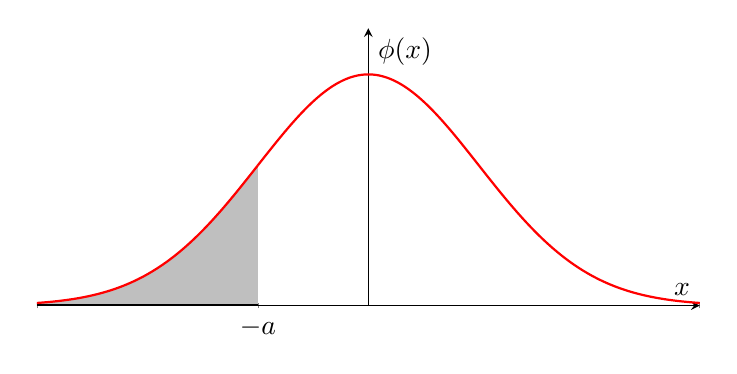
\begin{tikzpicture}[yscale=0.5]
	\begin{axis}[
    		axis lines = center,
		xmax=3,
		xmin=-3,
		ymax=1.2,
		ymin=0,
   		 xlabel = \( x \),
   		 ylabel = {\( \phi(x) \)},
		 xtick={-3,-1,0,3},
    		 xticklabels={$$, $-a$},
		 ytick={1},
		 yticklabels={},
		]
		 \node (some node) at (100,150) (a) {};
		  \node (some node) at (150,200) (c) {};
	\addplot[name path=A,samples=500,domain=-3:-1, color=red, style=thick]{e^(-0.5*x^2)};
	\addplot[samples=500,domain=-1:3, color=red, style=thick]{e^(-0.5*x^2)};
	\addplot[name path=B,thick, samples=50, smooth,domain=-3:1,black] coordinates {(-3,0)(-1,0)};
	\addplot[gray!50] fill between[of=A and B];
	\addplot [only marks] table {
};
	\end{axis}
	\end{tikzpicture}
	\end{center}

	Geometrically, however, we may see that this is equivalent to finding the shaded area here:
	
		\begin{center}
	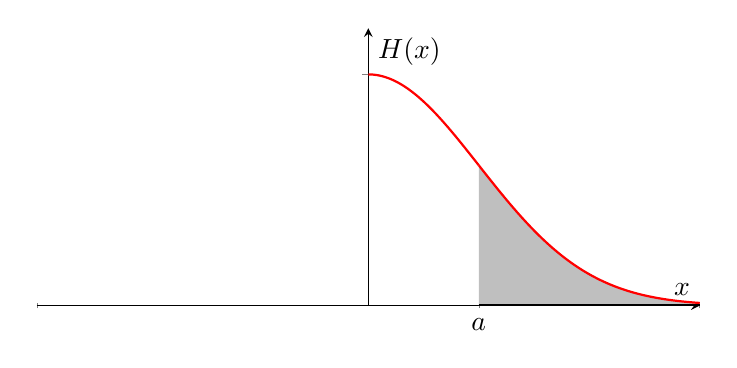
\begin{tikzpicture}[yscale=0.5]
	\begin{axis}[
    		axis lines = center,
		xmax=3,
		xmin=-3,
		ymax=1.2,
		ymin=0,
   		 xlabel = \( x \),
   		 ylabel = {\( H(x) \)},
		 xtick={-3,0,1,3},
    		 xticklabels={$$,$$, $a$},
		 ytick={1},
		 yticklabels={},
		]
		 \node (some node) at (100,150) (a) {};
		  \node (some node) at (150,200) (c) {};
	\addplot[samples=500,domain=0:1, color=red, style=thick]{e^(-0.5*x^2)};
	\addplot[name path=A,samples=500,domain=1:3, color=red, style=thick]{e^(-0.5*x^2)};
	\addplot[name path=B,thick, samples=50, smooth,domain=1:3,black] coordinates {(1,0)(3,0)};
	\addplot[gray!50] fill between[of=A and B];
	\addplot [only marks] table {
};
	\end{axis}
	\end{tikzpicture}
	\end{center}
	
	And so we can conclude 
	
	\[ \Phi(-a) = \frac{1}{2} - H(a) \]
	
	In a similar line of argument, if we wish to tabulate $\Phi(a) = P(X < a)$, then its relationship to $H(x)$ is given by
	
	\[ \Phi(a) = \frac{1}{2} + H(a) \]

	\begin{enumerate}
	%Question 9.35(a)
	\item  \begin{tcolorbox}[
	  colback=Cerulean!5!white,
	  colframe=Cerulean!75!black]
	\textbf{$\bm{P[|X| > 2]}$}
	\end{tcolorbox}
	
	Equivalently, we determine $P(X > 2) + P(X < -2)$. Note that $2, -2$ need to be normalized for the argument of $H(x)$. We have
	
	\begin{align*}
	P(X > 2) &= 1 - P(X < 2) = 1 - \bigg( \frac{1}{2} + H \bigg( \frac{2-1}{2} \bigg) \bigg) = \frac{1}{2} - H \bigg( \frac{1}{2} \bigg) \\
	P(X < -2) &= \frac{1}{2} - H \bigg( -\bigg( \frac{-2 - 1}{2} \bigg) \bigg) = \frac{1}{2} - H \bigg( \frac{3}{2} \bigg) \\
	\implies P[|X| > 2] &= \boxed{ 1 - [H(1/2) + H(3/2)] }
	\end{align*}
	
	%Question 9.35(b)
	\item  \begin{tcolorbox}[
	  colback=Cerulean!5!white,
	  colframe=Cerulean!75!black]
	\textbf{$\bm{P[X < 0]}$}
	\end{tcolorbox}
	
	By the above,
	
	\[ P(X < 0) = \Phi(-1/2) = \boxed{ \frac{1}{2} - H(1/2) } \]
	\end{enumerate}

\newpage
%Question 9.36
\item  \begin{tcolorbox}[
  colback=Cerulean!5!white,
  colframe=Cerulean!75!black]
\textbf{Suppose that a satellite telemetering device receives two kinds of signals which may be recorded as real numbers, say $\bm{X}$ and $\bm{Y}$. Assume that $\bm{X}$ and $\bm{Y}$ are independent, continuous random variables with pdf's $\bm{f}$ and $\bm{g}$, respectively. Suppose that during any specified period of time only one of these signals may be received and hence transmitted back to earth, namely that signal which arrives first. Assume furthermore that the signal giving rise to the value of $\bm{X}$ arrives first with probability $\bm{p}$ and hence the signal giving rise to $\bm{Y}$ arrives first with probability $\bm{1-p}$. Let $\bm{Z}$ denote the random variable whose value is actually received and transmitted.}
\end{tcolorbox}

	\begin{enumerate}
	%Question 9.36(a)
	\item  \begin{tcolorbox}[
	  colback=Cerulean!5!white,
	  colframe=Cerulean!75!black]
	\textbf{Express the pdf of $\bm{Z}$ in terms of $\bm{f}$ and $\bm{g}$.}
	\end{tcolorbox}
	
	The intuition is to view the events corresponding to $X$ and $Y$ as mutually exclusive. Either signal $X$ or $Y$ arrives, but not both. The probability that the value of $Z$ falls within, say, $[a,b]$, must be given by either
	
	\[ p \int^b_a f(x) \ dx \]
	
	or
	
	\[ (1-p) \int^b_a g(y) \ dy \]
	
	Thus, the probability distribution of the union of two mutually exclusive events must be given by
	
	\[ \boxed{ h(z) = p f(x) + (1-p) g(y) } \]
	
	which is a mixture of two normal distributions. The Kolmogorov axioms can be easily verified. By premise, we must have $f(x), g(y) \geq 0$, and $p, 1-p \geq 0$, so we must have $h(z) \geq 0$. Lastly,
	
	\[ p \int^{+\infty}_{-\infty} f(x) \ dx + (1-p) \int^{+\infty}_{-\infty} g(y) \ dy = p + 1 - p = 1 \quad \implies \quad \int^{+\infty}_{-\infty} h(z) \ dz = 1 \]
	
	%Question 9.36(b)
	\item  \begin{tcolorbox}[
	  colback=Cerulean!5!white,
	  colframe=Cerulean!75!black]
	\textbf{Express $\bm{E[Z]}$ in terms of $\bm{E[X]}$ and $\bm{E[Y]}$.}
	\end{tcolorbox}
	
	Since $Z$ takes on all of the values $X$ and $Y$ do, namely the reals, we can write
	
	\begin{align*}
	E[Z] &= \int^{+\infty}_{-\infty} z h(z) \ dz = p \int^{+\infty}_{-\infty} x f(x) \ dx + (1-p) \int^{+\infty}_{-\infty} y g(y) \ dy \\
	&= \boxed{p E[X] + (1-p) E[Y]}
	\end{align*}
	
	Intuitively, the expectation of $Z$ is a weighted average of the expectations of $X$ and $Y$.
	
	%Question 9.36(c)
	\item  \begin{tcolorbox}[
	  colback=Cerulean!5!white,
	  colframe=Cerulean!75!black]
	\textbf{Express $\bm{V[Z]}$ in terms of $\bm{V[X]}$ and $\bm{V[Y]}$.}
	\end{tcolorbox}
	
	We derive
	
	\begin{align*}
	V[Z] &= E[Z^2] - E[Z]^2 \\
	&= (p E[X^2] + (1-p)E[Y^2]) - (p E[X] + (1-p) E[Y])^2 \\
	&= (p E[X^2] + (1-p)E[Y^2]) - (p^2 E[X]^2 + 2p(1-p) E[X] E[Y] + (1-p)^2 E[Y]^2) \\
	&= p E[X^2] + E[Y^2] - p E[Y^2] - p^2 E[X]^2 - 2p E[X] E[Y] + 2p^2 E[X] E[Y] - E[Y]^2 + 2p E[Y]^2 - p^2 E[Y]^2
	\end{align*}
	
	Now, using the facts that $\sigma^2_X = E[X^2] - E[X]^2$ and $\sigma^2_Y = E[Y^2] - E[Y]^2$, we proceed as follows:
	
	\begin{align*}
	&= \sigma^2_Y + p(E[X^2] - 2E[X] E[Y] + 2E[Y]^2 - E[Y^2]) - p^2 (E[X]^2 - 2E[X] E[Y] + E[Y]^2) \\
	&= \sigma^2_Y + p(\sigma^2_X + E[X]^2 - 2E[X] E[Y] + E[Y]^2 - \sigma^2_Y) - p^2 (E[X] - E[Y])^2 \\
	&= \boxed{\sigma^2_Y + p(\sigma^2_X - \sigma^2_Y) + p(1-p) (\mu_x - \mu_y)^2}
	\end{align*}
	
	%Question 9.36(d)
	\item  \begin{tcolorbox}[
	  colback=Cerulean!5!white,
	  colframe=Cerulean!75!black]
	\textbf{Suppose that $\bm{X}$ has distribution $\bm{N(2,4)}$ and that $\bm{Y}$ has distribution $\bm{N(3,3)}$. If $\bm{p = \frac{2}{3}}$, evaluate $\bm{P(Z > 2)}$.}
	\end{tcolorbox}
	
	We calculate
	
	\[ P(Z > 2) = \int^{+\infty}_2 h(z) \ dz = \frac{2}{3} (1 - \Phi(0)) + \frac{1}{3} (1 - \Phi(- 1/\sqrt{3})) \approx \boxed{0.573} \]
	
	%Question 9.36(e)
	\item  \begin{tcolorbox}[
	  colback=Cerulean!5!white,
	  colframe=Cerulean!75!black]
	\textbf{Suppose that $\bm{X}$ and $\bm{Y}$ have distributions $\bm{N(\mu_1, \sigma^2_1)}$ and $\bm{N(\mu_2, \sigma^2_2)}$, respectively. Show that if $\bm{\mu_1 = \mu_2}$, the distribution of $\bm{Z}$ is ``uni-modal," that is, the pdf of $\bm{Z}$ has a unique relative maximum.}
	\end{tcolorbox}
	
	Our plan of attack will be to find the local maxima of $h(z)$, which will yield our points of modality. Appealing to the aforementioned logic that $X, Y$ effectively take on the same values as $Z$ (the reals), our task is to derive
	
	\[ \frac{d h(z)}{dz} = p \frac{d f(x)}{dx} + (1-p) \frac{d g(y)}{dy} \]
	
	where
	
	\begin{align*}
	p \frac{d f(x)}{dx} &= p \frac{1}{\sqrt{2\pi} \sigma_1} \frac{d}{dx} \exp \bigg[ -\frac{1}{2} \bigg( \frac{x-\mu_1}{\sigma_1} \bigg)^2 \bigg] = -p \frac{1}{\sqrt{2\pi} \sigma^3_1} (x-\mu_1) \exp  \bigg[ -\frac{1}{2} \bigg( \frac{x-\mu_1}{\sigma_1} \bigg)^2 \bigg] \\
	(1-p) \frac{d g(y)}{dy} &= (1-p) \frac{1}{\sqrt{2\pi} \sigma_2} \frac{d}{dy} \exp \bigg[ -\frac{1}{2} \bigg( \frac{y-\mu_2}{\sigma_2} \bigg)^2 \bigg] = -(1-p) \frac{1}{\sqrt{2\pi} \sigma^3_2} (y-\mu_2) \exp  \bigg[ -\frac{1}{2} \bigg( \frac{y-\mu_2}{\sigma_2} \bigg)^2 \bigg] \\
	\end{align*}
	
	Now, to find the local maxima, we set $dh(z) / dz = 0$. Therefore we must have
	
	\[ \frac{d h(z)}{dz} = \frac{1}{\sqrt{2\pi}} \bigg( \frac{p}{ \sigma^3_1} (x-\mu_1) \exp  \bigg[ -\frac{1}{2} \bigg( \frac{x-\mu_1}{\sigma_1} \bigg)^2 \bigg] + \bigg( \frac{1-p}{ \sigma^3_2} \bigg) (y-\mu_2) \exp  \bigg[ -\frac{1}{2} \bigg( \frac{y-\mu_2}{\sigma_2} \bigg)^2 \bigg] \bigg) = 0 \]
	
	An important note here is that it is not readily apparent to us what values of $x,y$ render this mixture of normal distributions to have a uni- or bimodal distribution.\footnote{See this discussion on Cross Validated for more: \url{https://stats.stackexchange.com/questions/416204/why-is-a-mixture-of-two-normally-distributed-variables-only-bimodal-if-their-mea}}. We need not concern ourselves with the general case of when unimodality holds, however; we only ask what happens if we now impose the condition that $\mu_1 = \mu_2$. Substitute each $\mu_1, \mu_2$ with $\mu$ to get
	
	\[ \frac{d h(z)}{dz} = \frac{1}{\sqrt{2\pi}} \bigg( \frac{p}{ \sigma^3_1} (x-\mu) \exp  \bigg[ -\frac{1}{2} \bigg( \frac{x-\mu}{\sigma_1} \bigg)^2 \bigg] + \bigg( \frac{1-p}{ \sigma^3_2} \bigg) (y-\mu) \exp  \bigg[ -\frac{1}{2} \bigg( \frac{y-\mu}{\sigma_2} \bigg)^2 \bigg] \bigg) = 0 \]
	
	Since the exponential terms will never go to zero exactly, we need only look at the $x - \mu, y - \mu$ terms to conclude that $dh(z) / dz$ if and only if $x = y = \mu$ under the aforementioned constraint. Therefore, if $\mu_1 = \mu_2$, then the pdf of $Z$ is unimodal.
	
	\end{enumerate}

%Question 9.37
\item  \begin{tcolorbox}[
  colback=Cerulean!5!white,
  colframe=Cerulean!75!black]
\textbf{Assume that the number of accidents in a factory may be represented by a Poisson process averaging 2 accidents a week. What is the probability that}
\end{tcolorbox}

	\begin{enumerate}
	%Question 9.37(a)
	\item  \begin{tcolorbox}[
	  colback=Cerulean!5!white,
	  colframe=Cerulean!75!black]
	\textbf{the time from one accident to the next will be more than three days [\textit{Hint}: In (a), let $\bm{T =}$ time (in days) and compute $\bm{P(T > 3)}$.]}
	\end{tcolorbox}
	
	Note that 2 accidents per week implies there are $2/7$ accidents per day. Here, $t = 3$. By assuming a Poisson process, we can model this situation as an exponential distribution with parameter $\alpha = 2/7$. We use an exponential distribution because that tells us the probability of an event occurring for the first time. With this framing, we can intuitively see that when an accident happens, we say that is $t = 0$, and calculate $P(T > 3)$, or the probability that it takes more than three days for the next accident to happen (equivalently, the probability it takes more than three days for the \textit{first accident since the one at $t=0$ to occur}):
	
	\[ P(T > 3) = \int^{+\infty}_3 \frac{2}{7} e^{-2t/7} \ dt \approx \boxed{0.424} \]
	
	%Question 9.37(b)
	\item  \begin{tcolorbox}[
	  colback=Cerulean!5!white,
	  colframe=Cerulean!75!black]
	\textbf{the time from one accident to the third accident will be more than a week?}
	\end{tcolorbox}
	
	Here we use a Gamma distribution to model the scenario, as it tells us the probability of the $r$-th occurrence of an event happening in a given period of time. Framing the scenario as in the previous case where one accident happening is at $t = 0$, we calculate $P(T > 7)$ for $r = 2$, since the \textit{second} accident happening \textit{after} the first is the \textit{third overall}:
	
	\[ P(T > 7) = \int^{+\infty}_7 \frac{2/7}{\Gamma(2)} \bigg( \frac{2}{7} t \bigg) e^{-2t/7} \ dt \approx \boxed{0.406} \]
	\end{enumerate}

%Question 9.38
\item  \begin{tcolorbox}[
  colback=Cerulean!5!white,
  colframe=Cerulean!75!black]
\textbf{On the average a production process produces one defective item among every 300 manufactured. What is the probability that the \textit{third} defective item will appear [\textit{Hint}: Assume a Poisson process]:}
\end{tcolorbox}

	\begin{enumerate}
	%Question 9.38(a)
	\item  \begin{tcolorbox}[
	  colback=Cerulean!5!white,
	  colframe=Cerulean!75!black]
	\textbf{before 1000 pieces have been produced?}
	\end{tcolorbox}
	
	Assuming a Poisson process, the binomial distribution applies here as we wish to find the number of occurrences of defectives in a fixed number of items. Let $n = 999$, the number of pieces produced before reaching 1000. By premise, $p = 1/300$, and $X = k = $ the number of defectives made. Equivalently, we may calculate the complement of the probability that only zero, one, or two defectives are made in the first 999 items:
	
	\begin{align*}
	1 - P(X = 0,1,2) &= 1 - \sum^2_{k=0} \binom{999}{k} \bigg( \frac{1}{300} \bigg)^k \bigg( \frac{299}{300} \bigg)^{999-k} \\
	&= \boxed{0.647}
	\end{align*}
	
	%Question 9.38(b)
	\item  \begin{tcolorbox}[
	  colback=Cerulean!5!white,
	  colframe=Cerulean!75!black]
	\textbf{as the 1000th piece is produced?}
	\end{tcolorbox}
	
	We should be inspired to model this with the Pascal distribution, which tells us the odds of an event happening for the $r$-th time on the $k$-th repetition of a Bernoulli experiment (here, either the $i$-th item produced is defective or not). With $k = 1000, r = 3$, we calculate
	
	\[ P(Y = 1000) = \binom{999}{2} \bigg( \frac{1}{300} \bigg)^3 \bigg( \frac{299}{300} \bigg)^{997} \approx \boxed{0.00066} \]
	
	%Question 9.38(c)
	\item  \begin{tcolorbox}[
	  colback=Cerulean!5!white,
	  colframe=Cerulean!75!black]
	\textbf{after the 1000th piece has been produced?}
	\end{tcolorbox}
	
	In an analogous logic as part (a), we can equivalently calculate the event that zero, one, or two defectives were created in the first 1000 pieces:
	
	\[ P(X = 0, 1, 2) = \sum^2_{k = 0} \binom{1000}{k} \bigg( \frac{1}{300} \bigg)^k \bigg( \frac{299}{300} \bigg)^{1000-k} \approx \boxed{0.352} \]
	\end{enumerate}

\end{enumerate}

\end{document}